\documentclass[11pt]{article}
\usepackage[textwidth=18.0cm, textheight=23.0cm, top=2.0cm]{geometry}
\usepackage{pst-all}
\usepackage{amssymb}
\usepackage{tikz}
\usepackage{underscore}\begin{document}
\pagestyle{empty}


ClassName: \underline{\textbf{Class_07.2bp-39}}
\par
BinSize: \underline{\textbf{100 × 100}}
\par
ReduceSize: \underline{\textbf{100 × 100}}
\par
TypeNum: \underline{\textbf{79}}
\par
Num: \underline{\textbf{80}}
\par
OutS: \underline{\textbf{240000}}
\par
InS: \underline{\textbf{203651}}
\par
Rate: \underline{\textbf{0.849}}
\par
UB: \underline{\textbf{24}}
\par
LB0: \underline{\textbf{24}}
\par
LB: \underline{\textbf{24}}
\par
LBWithCut: \underline{\textbf{24}}
\par
NodeCut: \underline{\textbf{0}}
\par
ExtendedNodeCnt: \underline{\textbf{1}}
\par
GenNodeCnt: \underline{\textbf{1}}
\par
PrimalNode: \underline{\textbf{0}}
\par
ColumnCount: \underline{\textbf{24}}
\par
TotalCutCount: \underline{\textbf{0}}
\par
RootCutCount: \underline{\textbf{0}}
\par
LPSolverCnt: \underline{\textbf{1}}
\par
PricingSolverCnt: \underline{\textbf{0}}
\par
BranchAndBoundNum: \underline{\textbf{1}}
\par
isOpt: \underline{\textbf{true}}
\par
TimeOnPrimal: \underline{\textbf{0.000 s}}
\par
TimeOnPricing: \underline{\textbf{0.000 s}}
\par
TimeOnRmp: \underline{\textbf{0.062 s}}
\par
TotalTime: \underline{\textbf{0.125 s}}
\par
\newpage


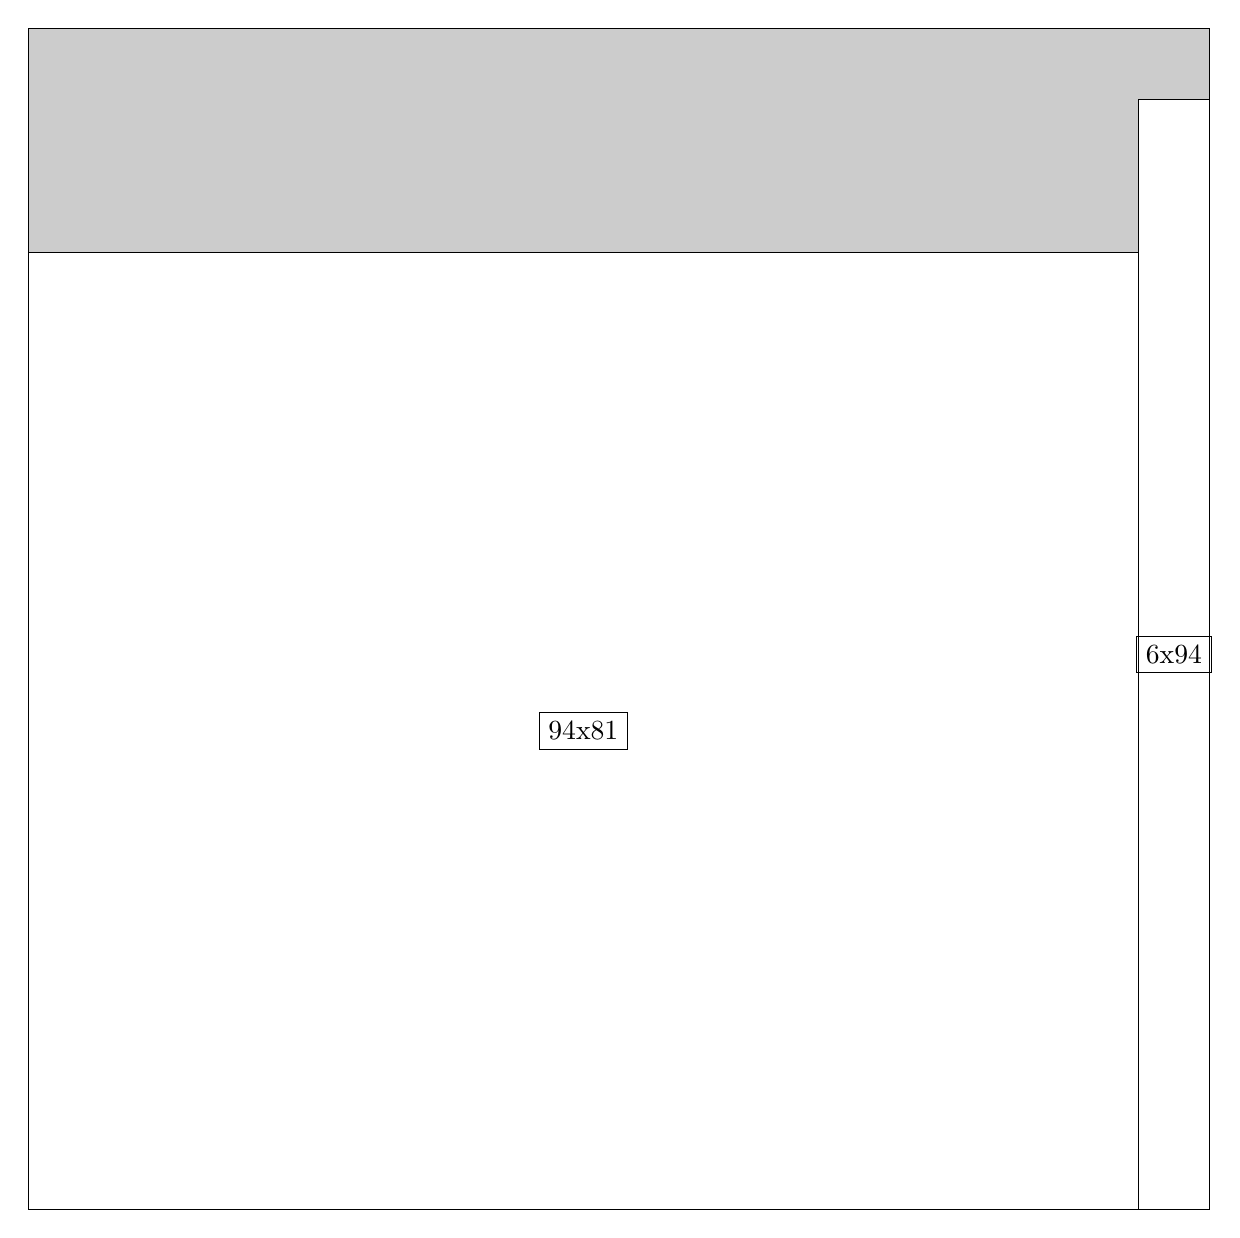
\begin{tikzpicture}[shorten >=1pt,scale=1.0,every node/.style={scale=1.0},->]
\tikzstyle{vertex}=[circle,fill=black!25,minimum size=14pt,inner sep=0pt]
\filldraw[fill=gray!40!white, draw=black] (0,0) rectangle (15.0,15.0);
\foreach \name/\x/\y/\w/\h in {94x81/0.0/0.0/14.1/12.15,6x94/14.1/0.0/0.8999999999999999/14.1}
\filldraw[fill=white!40!white, draw=black] (\x,\y) rectangle node[draw] (\name) {\name} ++(\w,\h);
\end{tikzpicture}


w =94 , h =81 , x =0 , y =0 , v =7614
\par
w =6 , h =94 , x =94 , y =0 , v =564
\par
\newpage


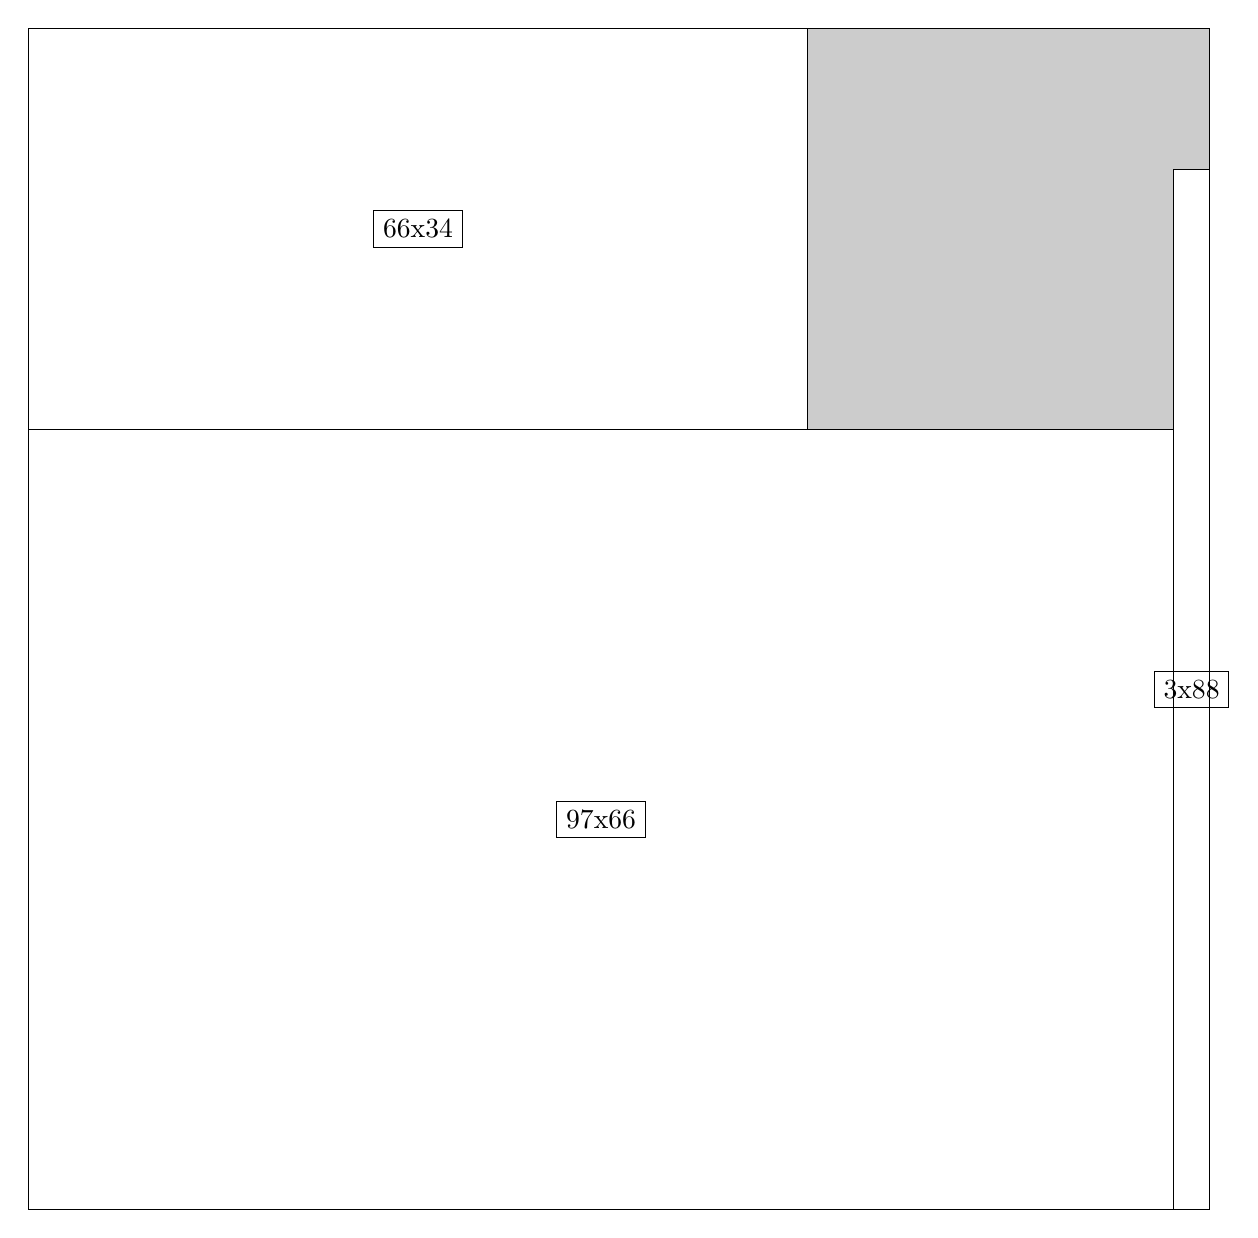
\begin{tikzpicture}[shorten >=1pt,scale=1.0,every node/.style={scale=1.0},->]
\tikzstyle{vertex}=[circle,fill=black!25,minimum size=14pt,inner sep=0pt]
\filldraw[fill=gray!40!white, draw=black] (0,0) rectangle (15.0,15.0);
\foreach \name/\x/\y/\w/\h in {97x66/0.0/0.0/14.549999999999999/9.9,66x34/0.0/9.9/9.9/5.1,3x88/14.549999999999999/0.0/0.44999999999999996/13.2}
\filldraw[fill=white!40!white, draw=black] (\x,\y) rectangle node[draw] (\name) {\name} ++(\w,\h);
\end{tikzpicture}


w =97 , h =66 , x =0 , y =0 , v =6402
\par
w =66 , h =34 , x =0 , y =66 , v =2244
\par
w =3 , h =88 , x =97 , y =0 , v =264
\par
\newpage


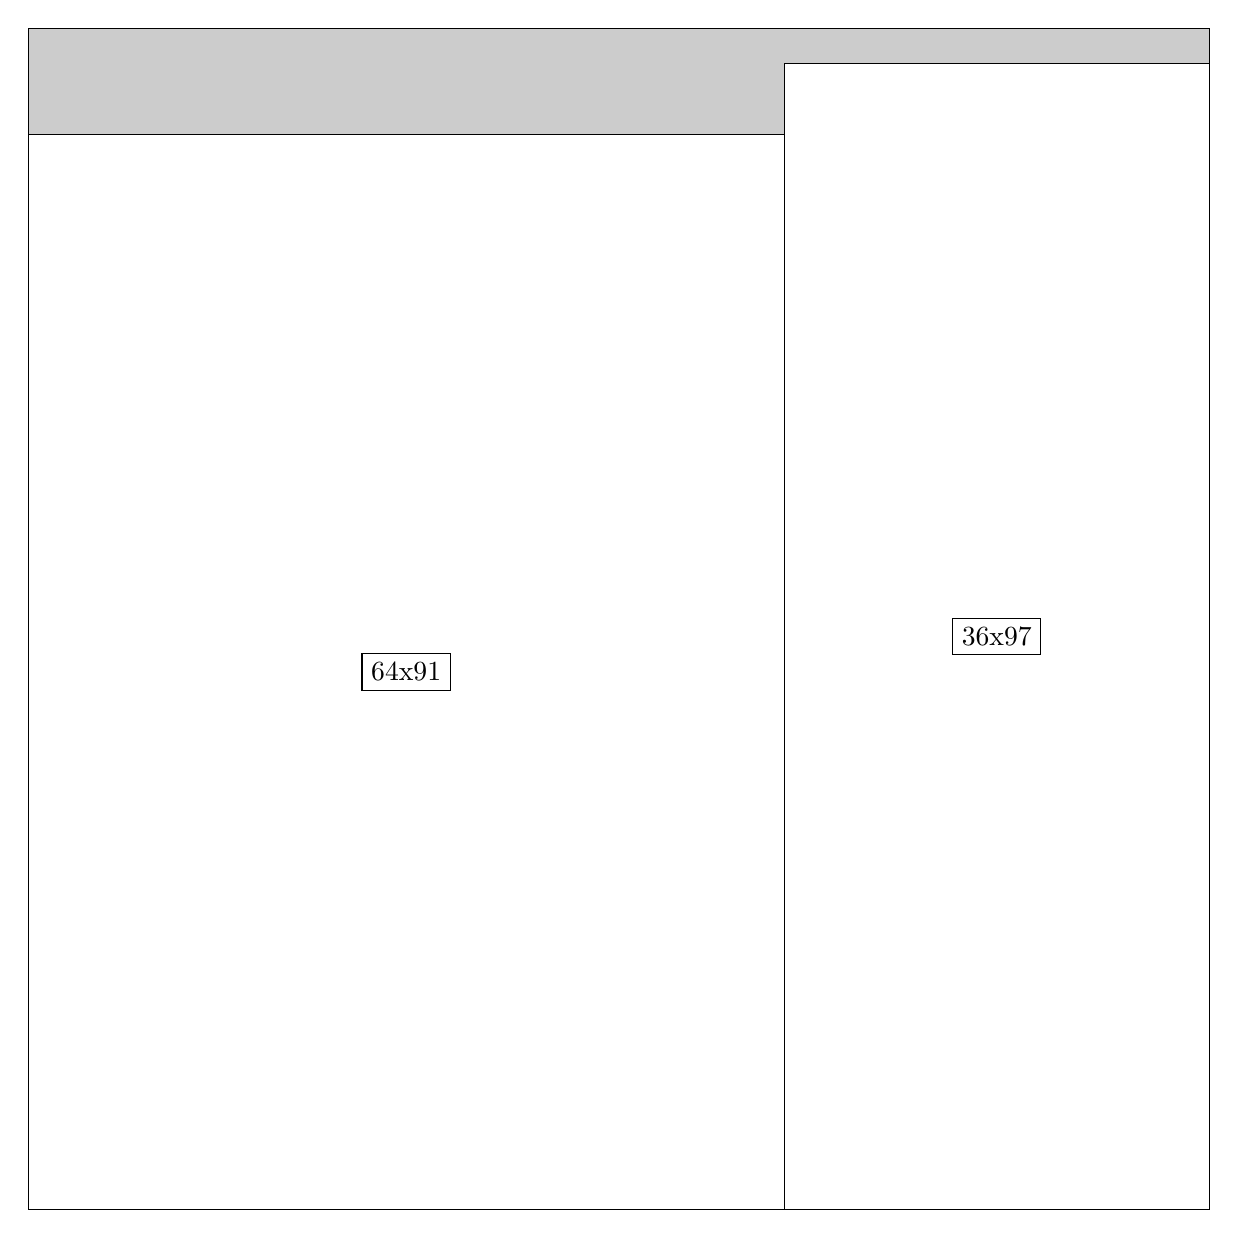
\begin{tikzpicture}[shorten >=1pt,scale=1.0,every node/.style={scale=1.0},->]
\tikzstyle{vertex}=[circle,fill=black!25,minimum size=14pt,inner sep=0pt]
\filldraw[fill=gray!40!white, draw=black] (0,0) rectangle (15.0,15.0);
\foreach \name/\x/\y/\w/\h in {64x91/0.0/0.0/9.6/13.65,36x97/9.6/0.0/5.3999999999999995/14.549999999999999}
\filldraw[fill=white!40!white, draw=black] (\x,\y) rectangle node[draw] (\name) {\name} ++(\w,\h);
\end{tikzpicture}


w =64 , h =91 , x =0 , y =0 , v =5824
\par
w =36 , h =97 , x =64 , y =0 , v =3492
\par
\newpage


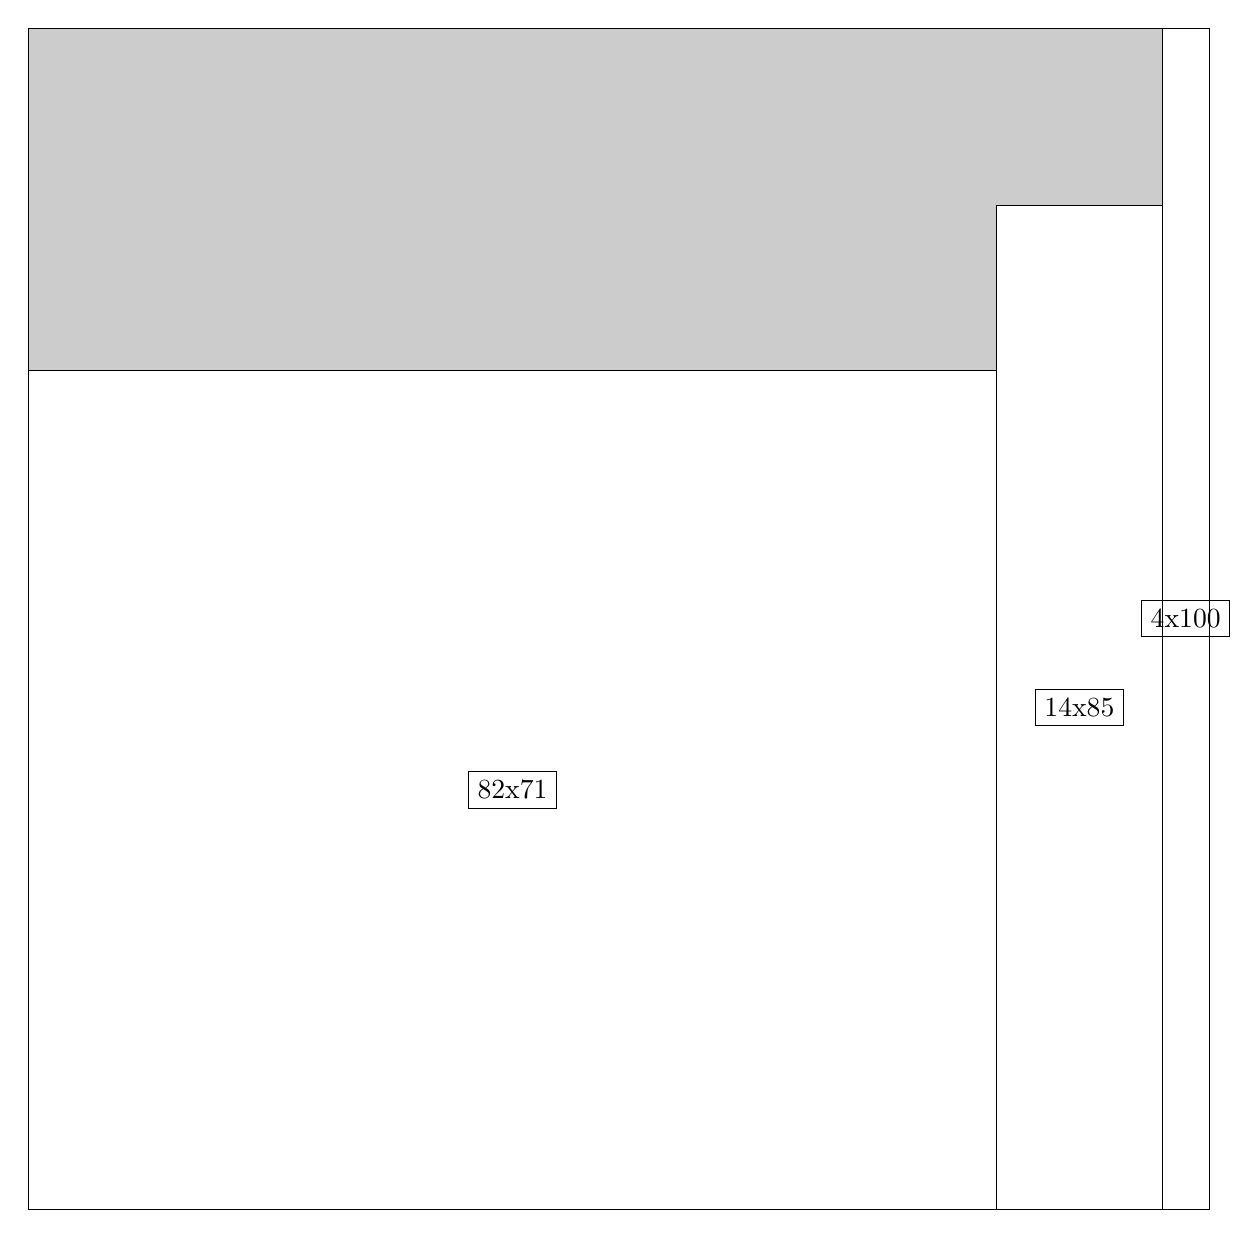
\begin{tikzpicture}[shorten >=1pt,scale=1.0,every node/.style={scale=1.0},->]
\tikzstyle{vertex}=[circle,fill=black!25,minimum size=14pt,inner sep=0pt]
\filldraw[fill=gray!40!white, draw=black] (0,0) rectangle (15.0,15.0);
\foreach \name/\x/\y/\w/\h in {82x71/0.0/0.0/12.299999999999999/10.65,14x85/12.299999999999999/0.0/2.1/12.75,4x100/14.399999999999999/0.0/0.6/15.0}
\filldraw[fill=white!40!white, draw=black] (\x,\y) rectangle node[draw] (\name) {\name} ++(\w,\h);
\end{tikzpicture}


w =82 , h =71 , x =0 , y =0 , v =5822
\par
w =14 , h =85 , x =82 , y =0 , v =1190
\par
w =4 , h =100 , x =96 , y =0 , v =400
\par
\newpage


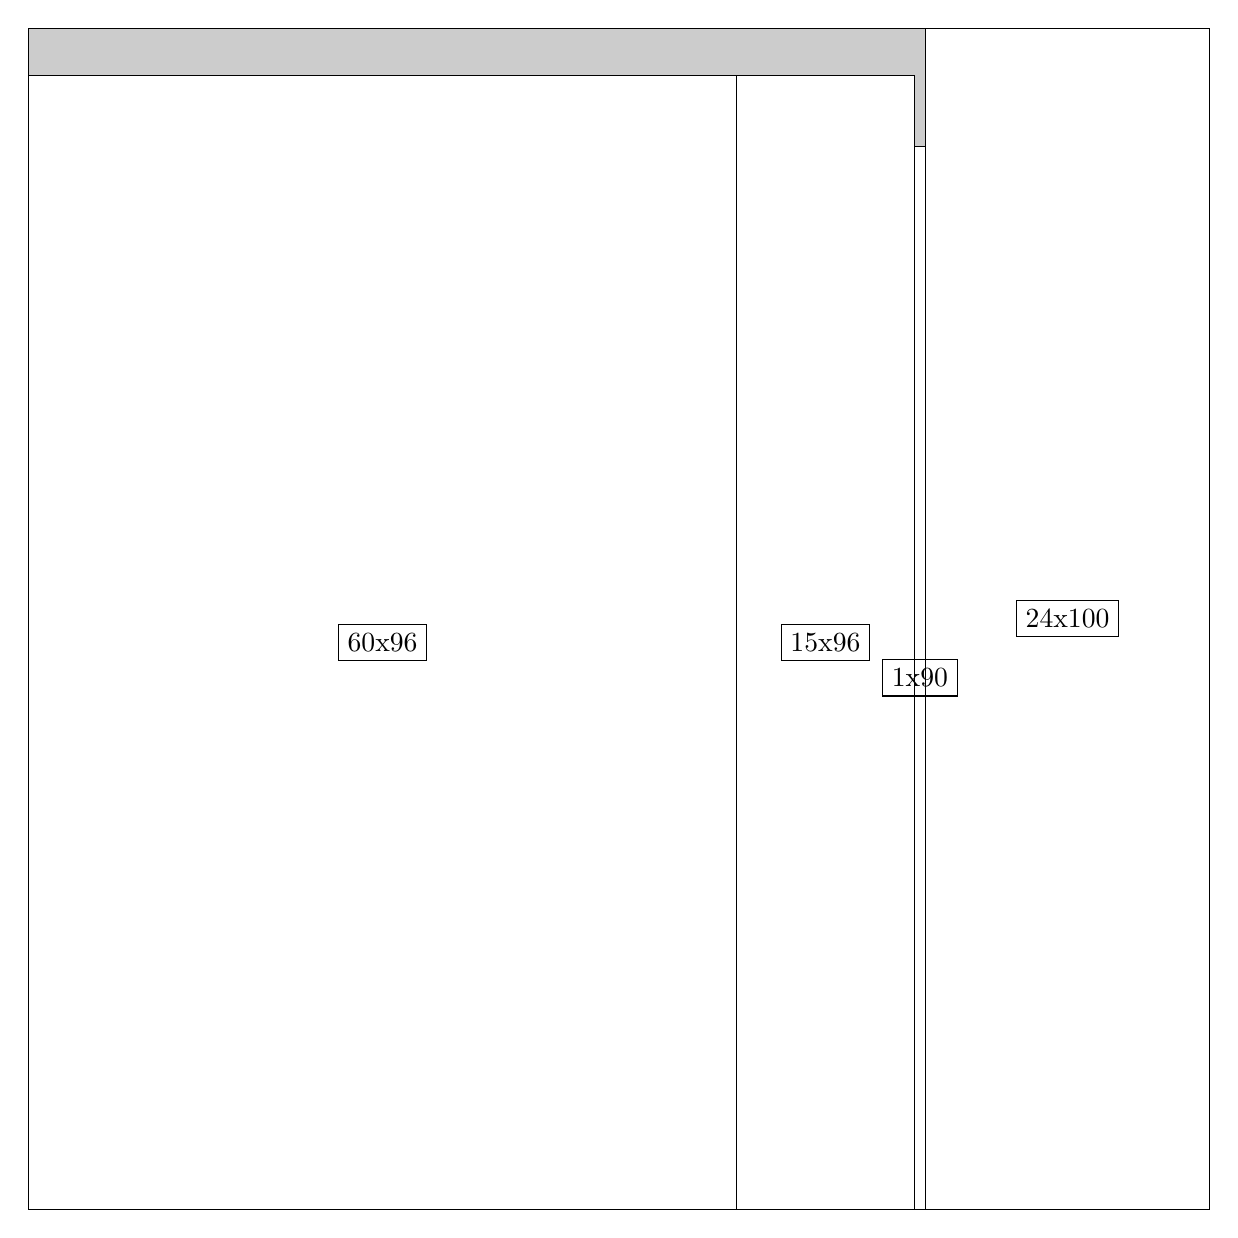
\begin{tikzpicture}[shorten >=1pt,scale=1.0,every node/.style={scale=1.0},->]
\tikzstyle{vertex}=[circle,fill=black!25,minimum size=14pt,inner sep=0pt]
\filldraw[fill=gray!40!white, draw=black] (0,0) rectangle (15.0,15.0);
\foreach \name/\x/\y/\w/\h in {60x96/0.0/0.0/9.0/14.399999999999999,24x100/11.4/0.0/3.5999999999999996/15.0,15x96/9.0/0.0/2.25/14.399999999999999,1x90/11.25/0.0/0.15/13.5}
\filldraw[fill=white!40!white, draw=black] (\x,\y) rectangle node[draw] (\name) {\name} ++(\w,\h);
\end{tikzpicture}


w =60 , h =96 , x =0 , y =0 , v =5760
\par
w =24 , h =100 , x =76 , y =0 , v =2400
\par
w =15 , h =96 , x =60 , y =0 , v =1440
\par
w =1 , h =90 , x =75 , y =0 , v =90
\par
\newpage


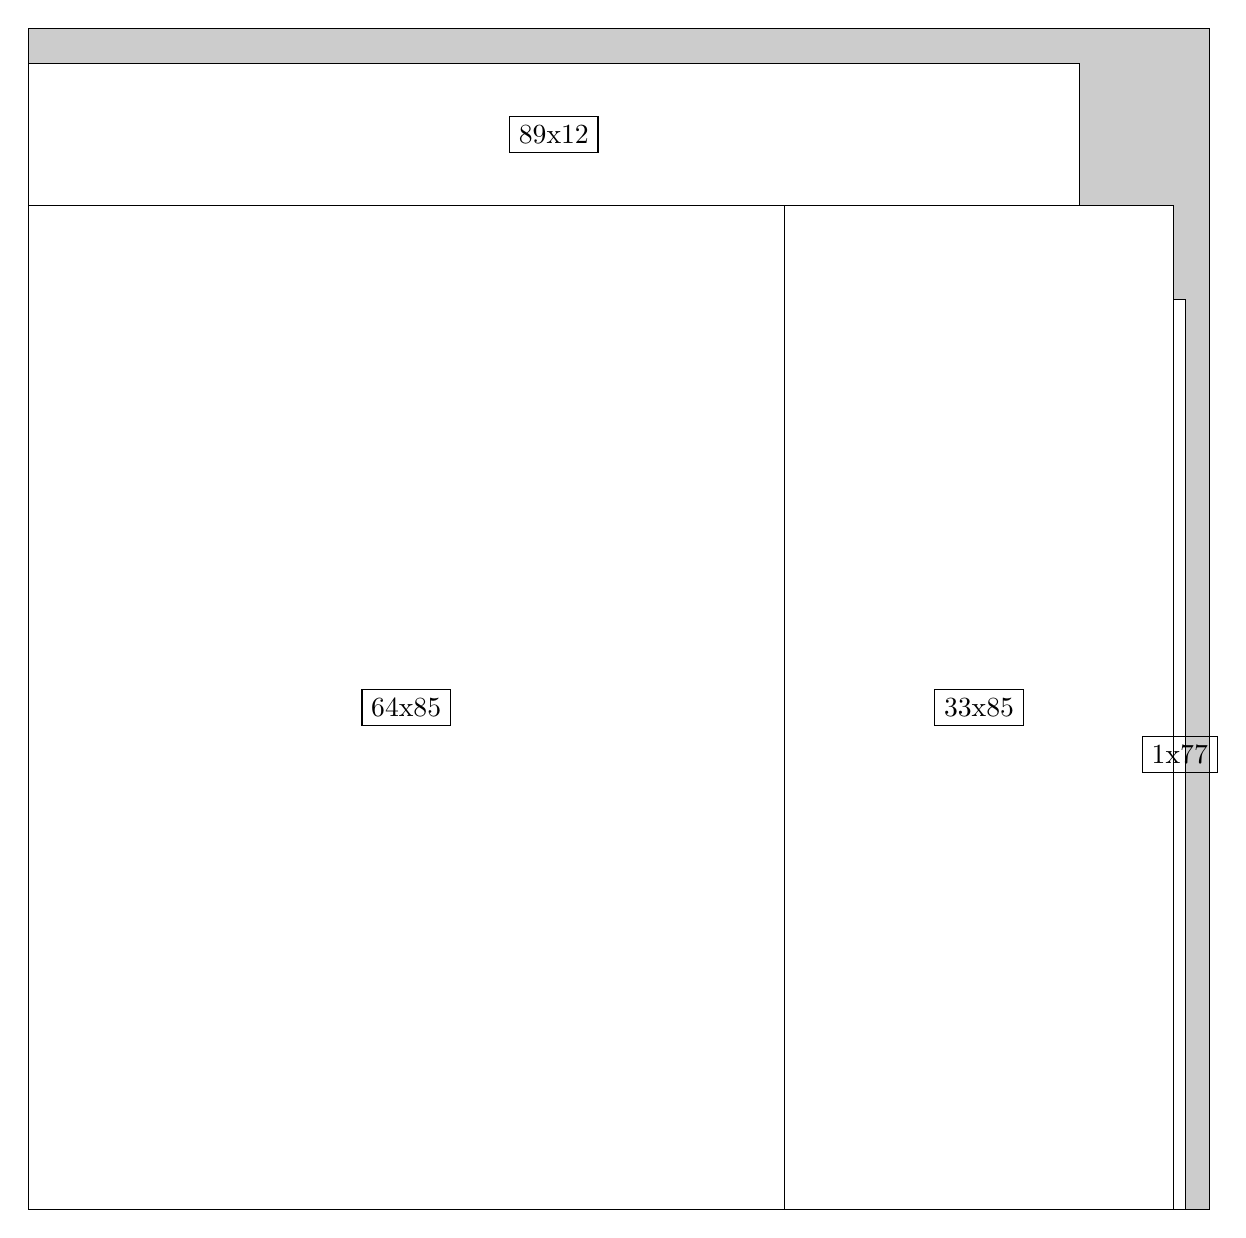
\begin{tikzpicture}[shorten >=1pt,scale=1.0,every node/.style={scale=1.0},->]
\tikzstyle{vertex}=[circle,fill=black!25,minimum size=14pt,inner sep=0pt]
\filldraw[fill=gray!40!white, draw=black] (0,0) rectangle (15.0,15.0);
\foreach \name/\x/\y/\w/\h in {64x85/0.0/0.0/9.6/12.75,33x85/9.6/0.0/4.95/12.75,89x12/0.0/12.75/13.35/1.7999999999999998,1x77/14.549999999999999/0.0/0.15/11.549999999999999}
\filldraw[fill=white!40!white, draw=black] (\x,\y) rectangle node[draw] (\name) {\name} ++(\w,\h);
\end{tikzpicture}


w =64 , h =85 , x =0 , y =0 , v =5440
\par
w =33 , h =85 , x =64 , y =0 , v =2805
\par
w =89 , h =12 , x =0 , y =85 , v =1068
\par
w =1 , h =77 , x =97 , y =0 , v =77
\par
\newpage


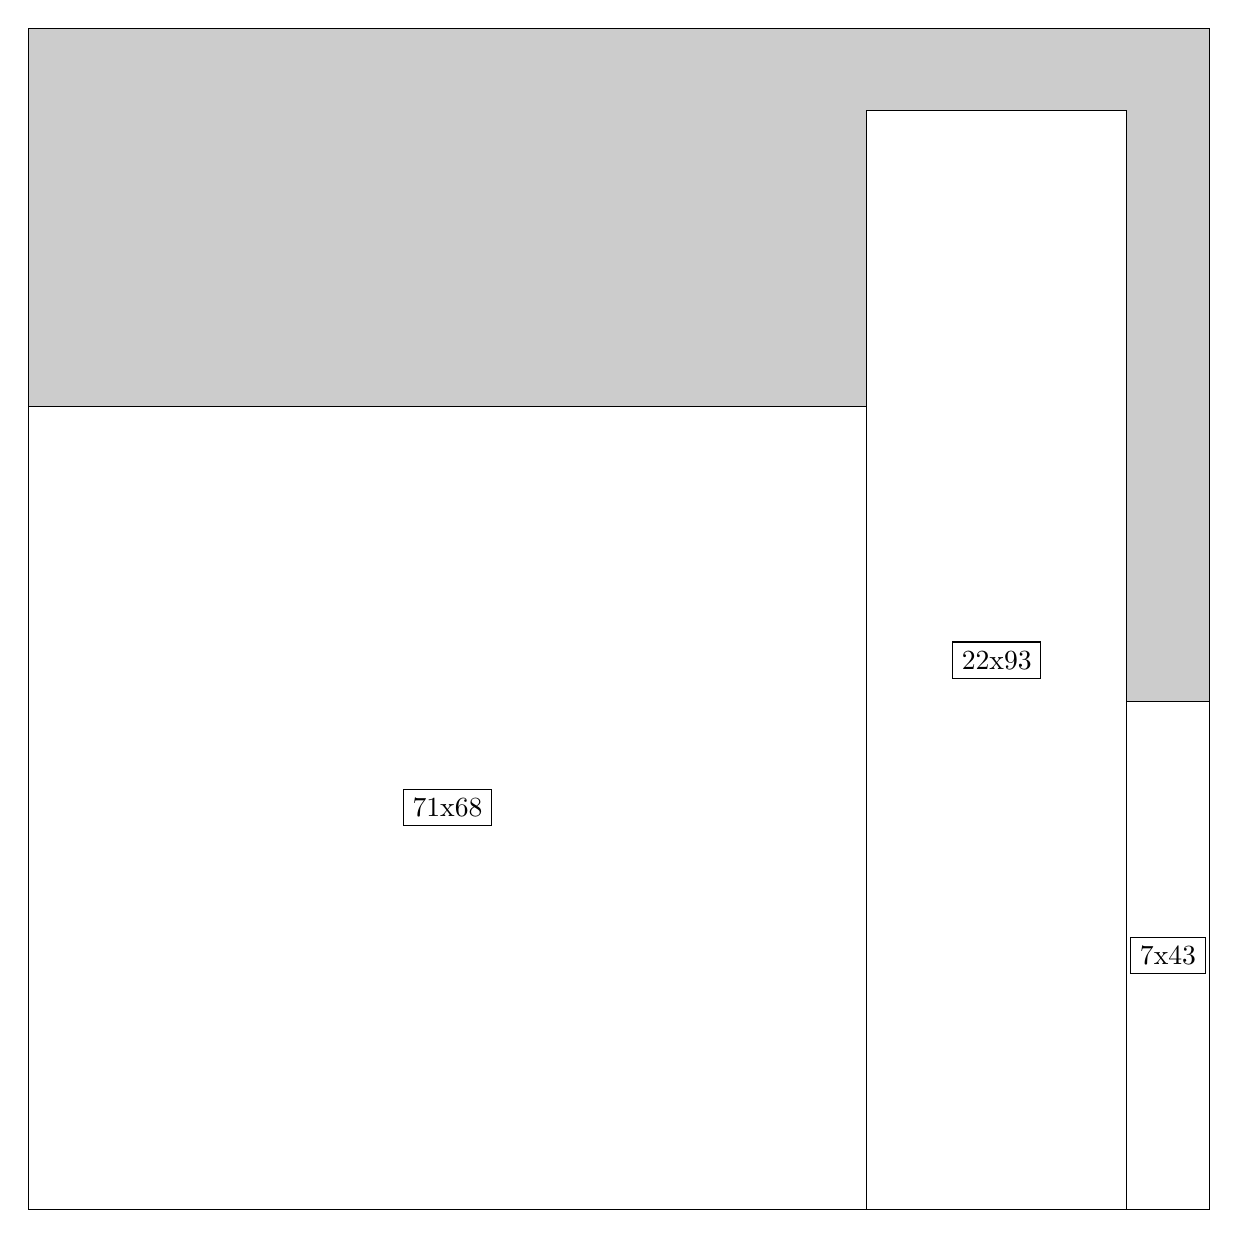
\begin{tikzpicture}[shorten >=1pt,scale=1.0,every node/.style={scale=1.0},->]
\tikzstyle{vertex}=[circle,fill=black!25,minimum size=14pt,inner sep=0pt]
\filldraw[fill=gray!40!white, draw=black] (0,0) rectangle (15.0,15.0);
\foreach \name/\x/\y/\w/\h in {71x68/0.0/0.0/10.65/10.2,22x93/10.65/0.0/3.3/13.95,7x43/13.95/0.0/1.05/6.45}
\filldraw[fill=white!40!white, draw=black] (\x,\y) rectangle node[draw] (\name) {\name} ++(\w,\h);
\end{tikzpicture}


w =71 , h =68 , x =0 , y =0 , v =4828
\par
w =22 , h =93 , x =71 , y =0 , v =2046
\par
w =7 , h =43 , x =93 , y =0 , v =301
\par
\newpage


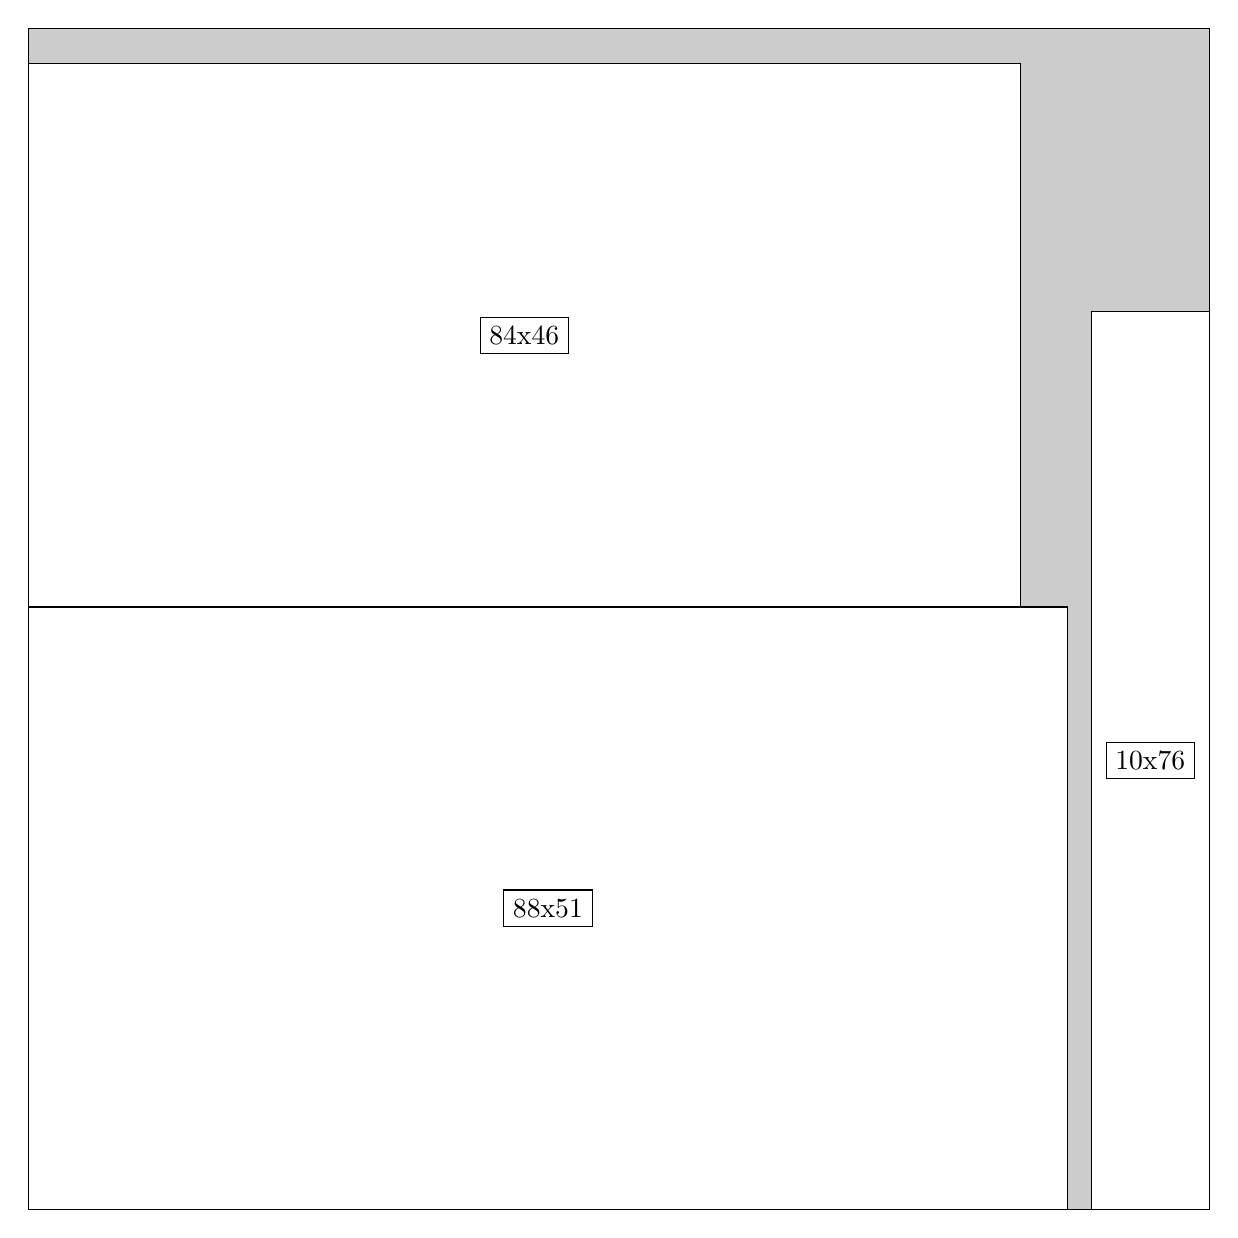
\begin{tikzpicture}[shorten >=1pt,scale=1.0,every node/.style={scale=1.0},->]
\tikzstyle{vertex}=[circle,fill=black!25,minimum size=14pt,inner sep=0pt]
\filldraw[fill=gray!40!white, draw=black] (0,0) rectangle (15.0,15.0);
\foreach \name/\x/\y/\w/\h in {88x51/0.0/0.0/13.2/7.6499999999999995,84x46/0.0/7.6499999999999995/12.6/6.8999999999999995,10x76/13.5/0.0/1.5/11.4}
\filldraw[fill=white!40!white, draw=black] (\x,\y) rectangle node[draw] (\name) {\name} ++(\w,\h);
\end{tikzpicture}


w =88 , h =51 , x =0 , y =0 , v =4488
\par
w =84 , h =46 , x =0 , y =51 , v =3864
\par
w =10 , h =76 , x =90 , y =0 , v =760
\par
\newpage


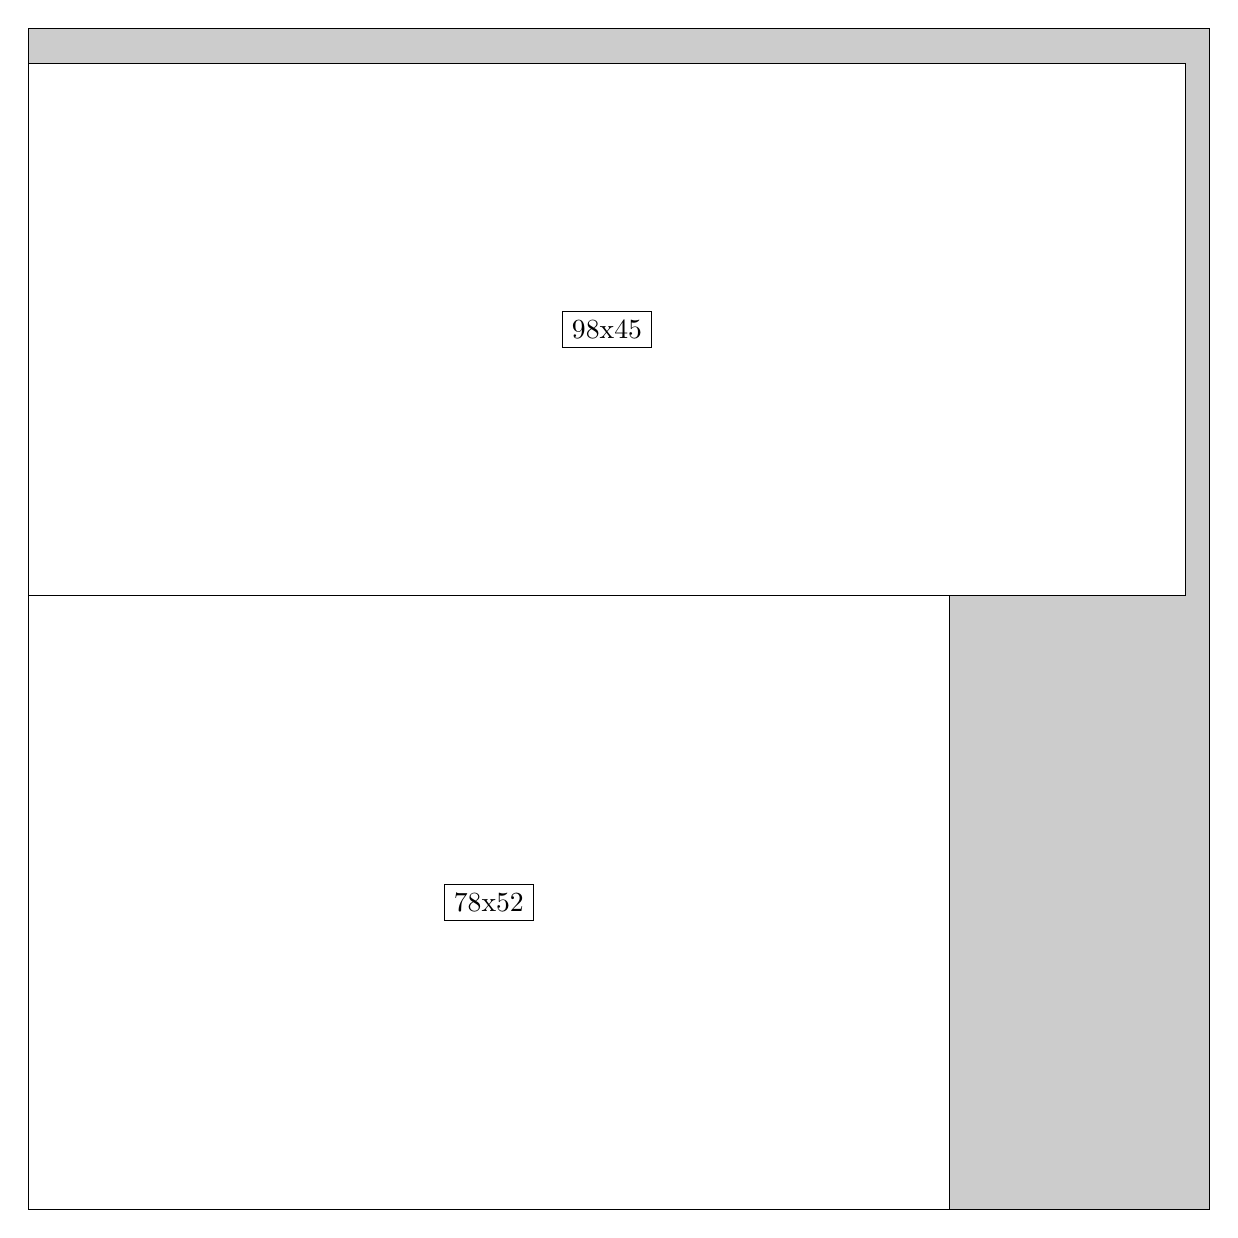
\begin{tikzpicture}[shorten >=1pt,scale=1.0,every node/.style={scale=1.0},->]
\tikzstyle{vertex}=[circle,fill=black!25,minimum size=14pt,inner sep=0pt]
\filldraw[fill=gray!40!white, draw=black] (0,0) rectangle (15.0,15.0);
\foreach \name/\x/\y/\w/\h in {98x45/0.0/7.8/14.7/6.75,78x52/0.0/0.0/11.7/7.8}
\filldraw[fill=white!40!white, draw=black] (\x,\y) rectangle node[draw] (\name) {\name} ++(\w,\h);
\end{tikzpicture}


w =98 , h =45 , x =0 , y =52 , v =4410
\par
w =78 , h =52 , x =0 , y =0 , v =4056
\par
\newpage


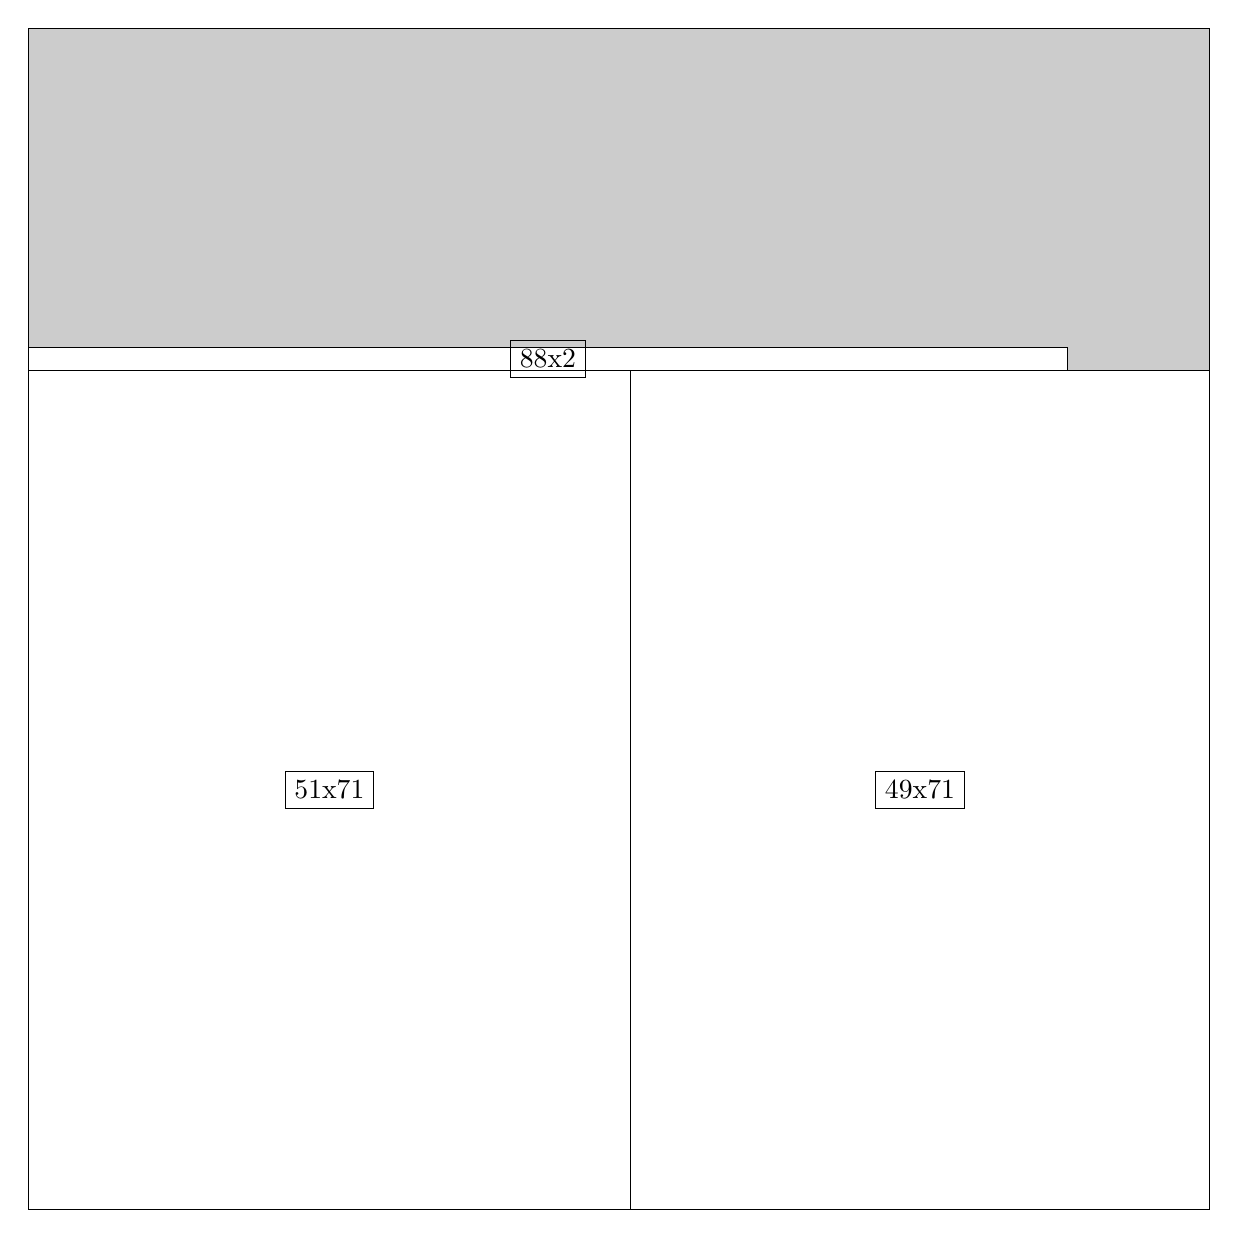
\begin{tikzpicture}[shorten >=1pt,scale=1.0,every node/.style={scale=1.0},->]
\tikzstyle{vertex}=[circle,fill=black!25,minimum size=14pt,inner sep=0pt]
\filldraw[fill=gray!40!white, draw=black] (0,0) rectangle (15.0,15.0);
\foreach \name/\x/\y/\w/\h in {51x71/0.0/0.0/7.6499999999999995/10.65,49x71/7.6499999999999995/0.0/7.35/10.65,88x2/0.0/10.65/13.2/0.3}
\filldraw[fill=white!40!white, draw=black] (\x,\y) rectangle node[draw] (\name) {\name} ++(\w,\h);
\end{tikzpicture}


w =51 , h =71 , x =0 , y =0 , v =3621
\par
w =49 , h =71 , x =51 , y =0 , v =3479
\par
w =88 , h =2 , x =0 , y =71 , v =176
\par
\newpage


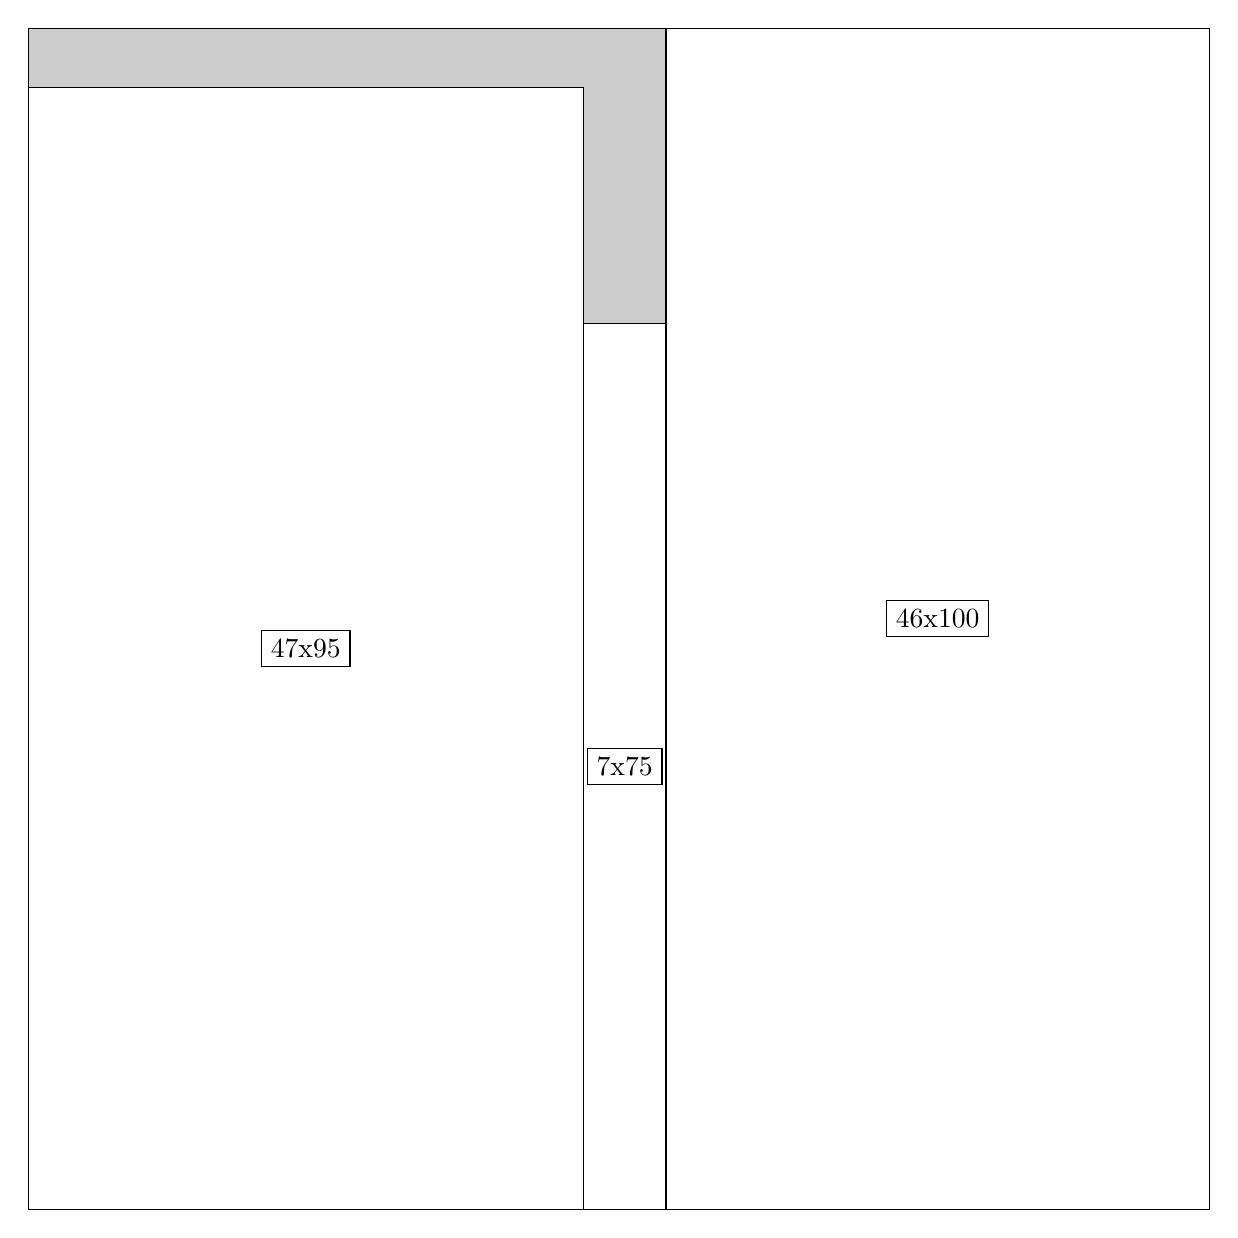
\begin{tikzpicture}[shorten >=1pt,scale=1.0,every node/.style={scale=1.0},->]
\tikzstyle{vertex}=[circle,fill=black!25,minimum size=14pt,inner sep=0pt]
\filldraw[fill=gray!40!white, draw=black] (0,0) rectangle (15.0,15.0);
\foreach \name/\x/\y/\w/\h in {46x100/8.1/0.0/6.8999999999999995/15.0,47x95/0.0/0.0/7.05/14.25,7x75/7.05/0.0/1.05/11.25}
\filldraw[fill=white!40!white, draw=black] (\x,\y) rectangle node[draw] (\name) {\name} ++(\w,\h);
\end{tikzpicture}


w =46 , h =100 , x =54 , y =0 , v =4600
\par
w =47 , h =95 , x =0 , y =0 , v =4465
\par
w =7 , h =75 , x =47 , y =0 , v =525
\par
\newpage


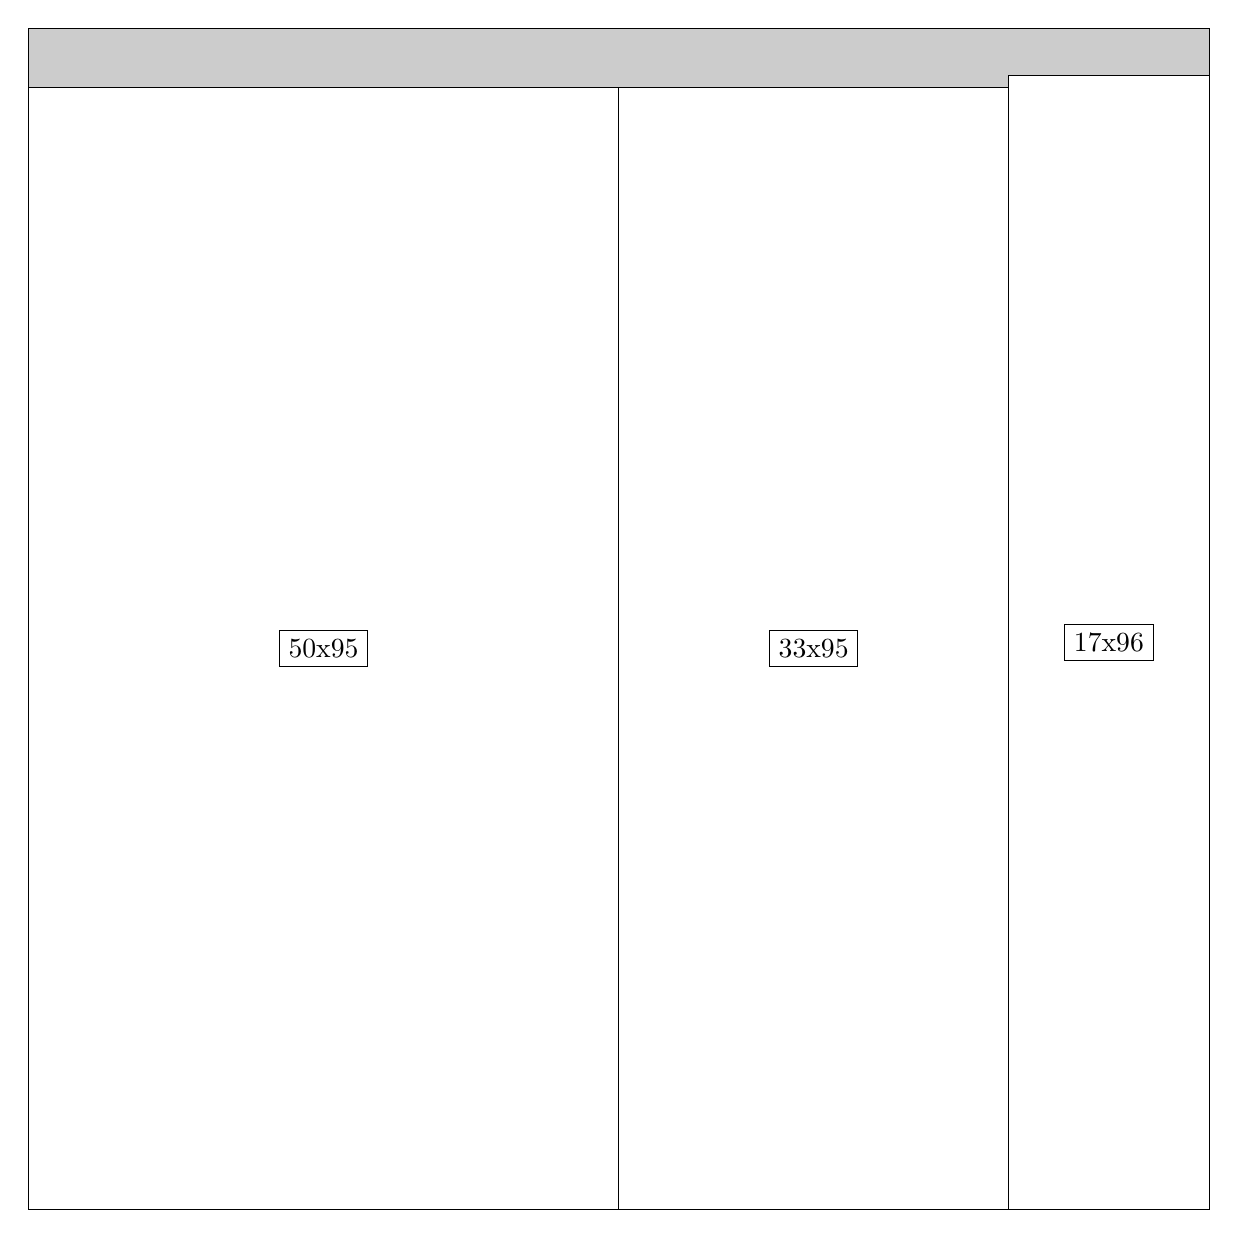
\begin{tikzpicture}[shorten >=1pt,scale=1.0,every node/.style={scale=1.0},->]
\tikzstyle{vertex}=[circle,fill=black!25,minimum size=14pt,inner sep=0pt]
\filldraw[fill=gray!40!white, draw=black] (0,0) rectangle (15.0,15.0);
\foreach \name/\x/\y/\w/\h in {50x95/0.0/0.0/7.5/14.25,33x95/7.5/0.0/4.95/14.25,17x96/12.45/0.0/2.55/14.399999999999999}
\filldraw[fill=white!40!white, draw=black] (\x,\y) rectangle node[draw] (\name) {\name} ++(\w,\h);
\end{tikzpicture}


w =50 , h =95 , x =0 , y =0 , v =4750
\par
w =33 , h =95 , x =50 , y =0 , v =3135
\par
w =17 , h =96 , x =83 , y =0 , v =1632
\par
\newpage


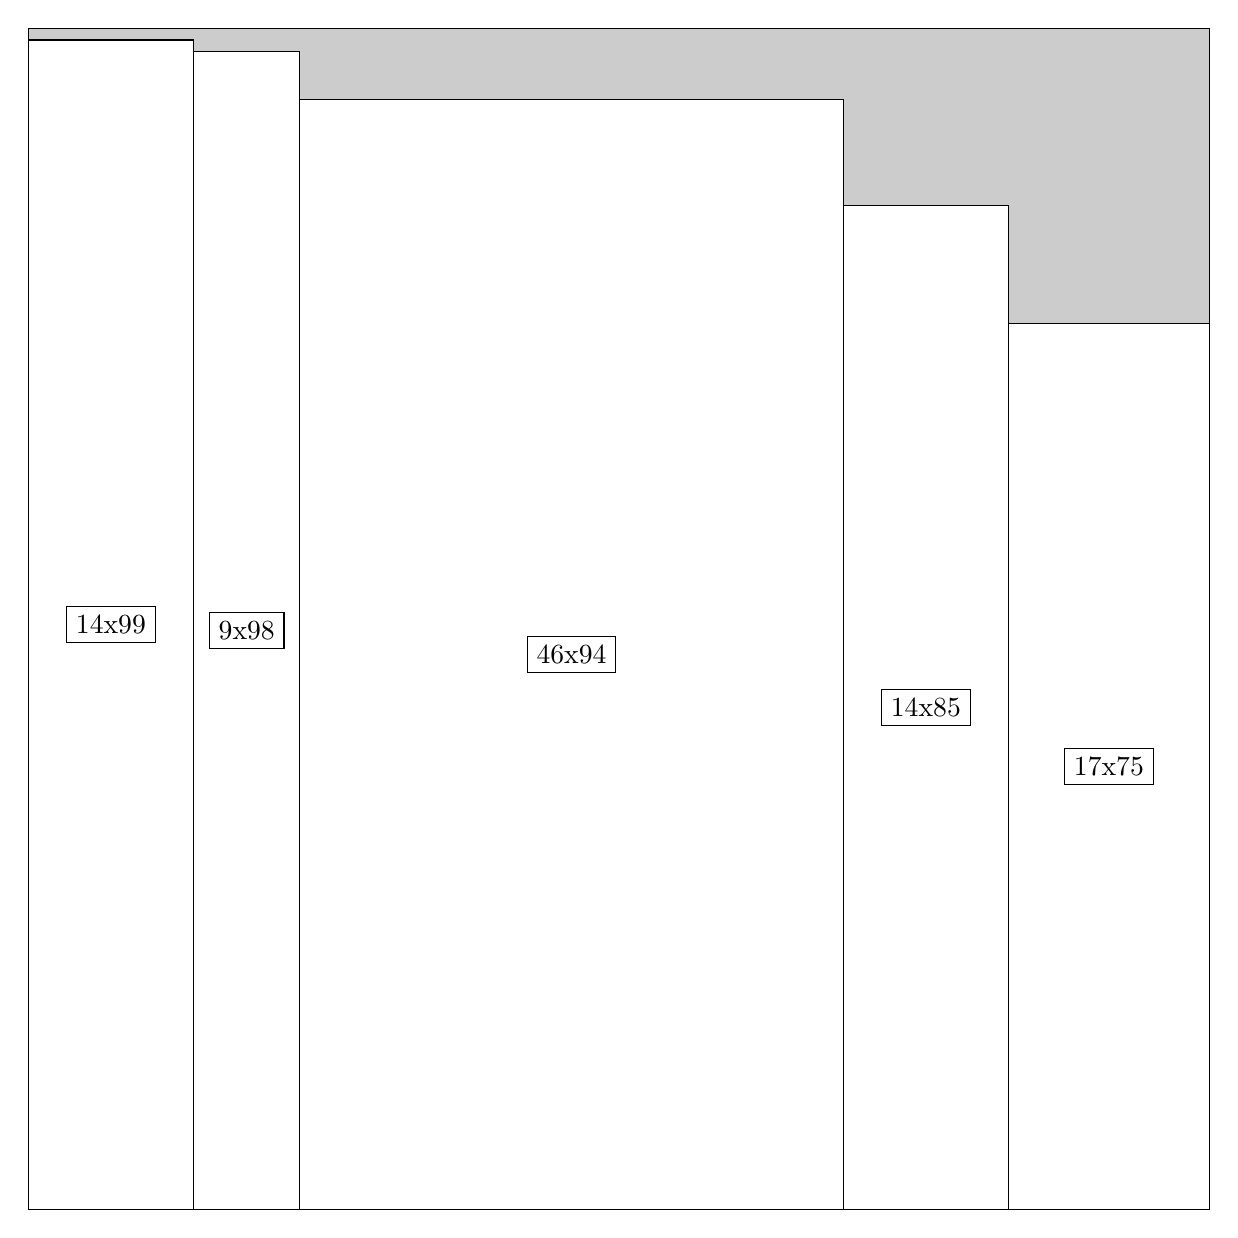
\begin{tikzpicture}[shorten >=1pt,scale=1.0,every node/.style={scale=1.0},->]
\tikzstyle{vertex}=[circle,fill=black!25,minimum size=14pt,inner sep=0pt]
\filldraw[fill=gray!40!white, draw=black] (0,0) rectangle (15.0,15.0);
\foreach \name/\x/\y/\w/\h in {46x94/3.4499999999999997/0.0/6.8999999999999995/14.1,14x99/0.0/0.0/2.1/14.85,17x75/12.45/0.0/2.55/11.25,14x85/10.35/0.0/2.1/12.75,9x98/2.1/0.0/1.3499999999999999/14.7}
\filldraw[fill=white!40!white, draw=black] (\x,\y) rectangle node[draw] (\name) {\name} ++(\w,\h);
\end{tikzpicture}


w =46 , h =94 , x =23 , y =0 , v =4324
\par
w =14 , h =99 , x =0 , y =0 , v =1386
\par
w =17 , h =75 , x =83 , y =0 , v =1275
\par
w =14 , h =85 , x =69 , y =0 , v =1190
\par
w =9 , h =98 , x =14 , y =0 , v =882
\par
\newpage


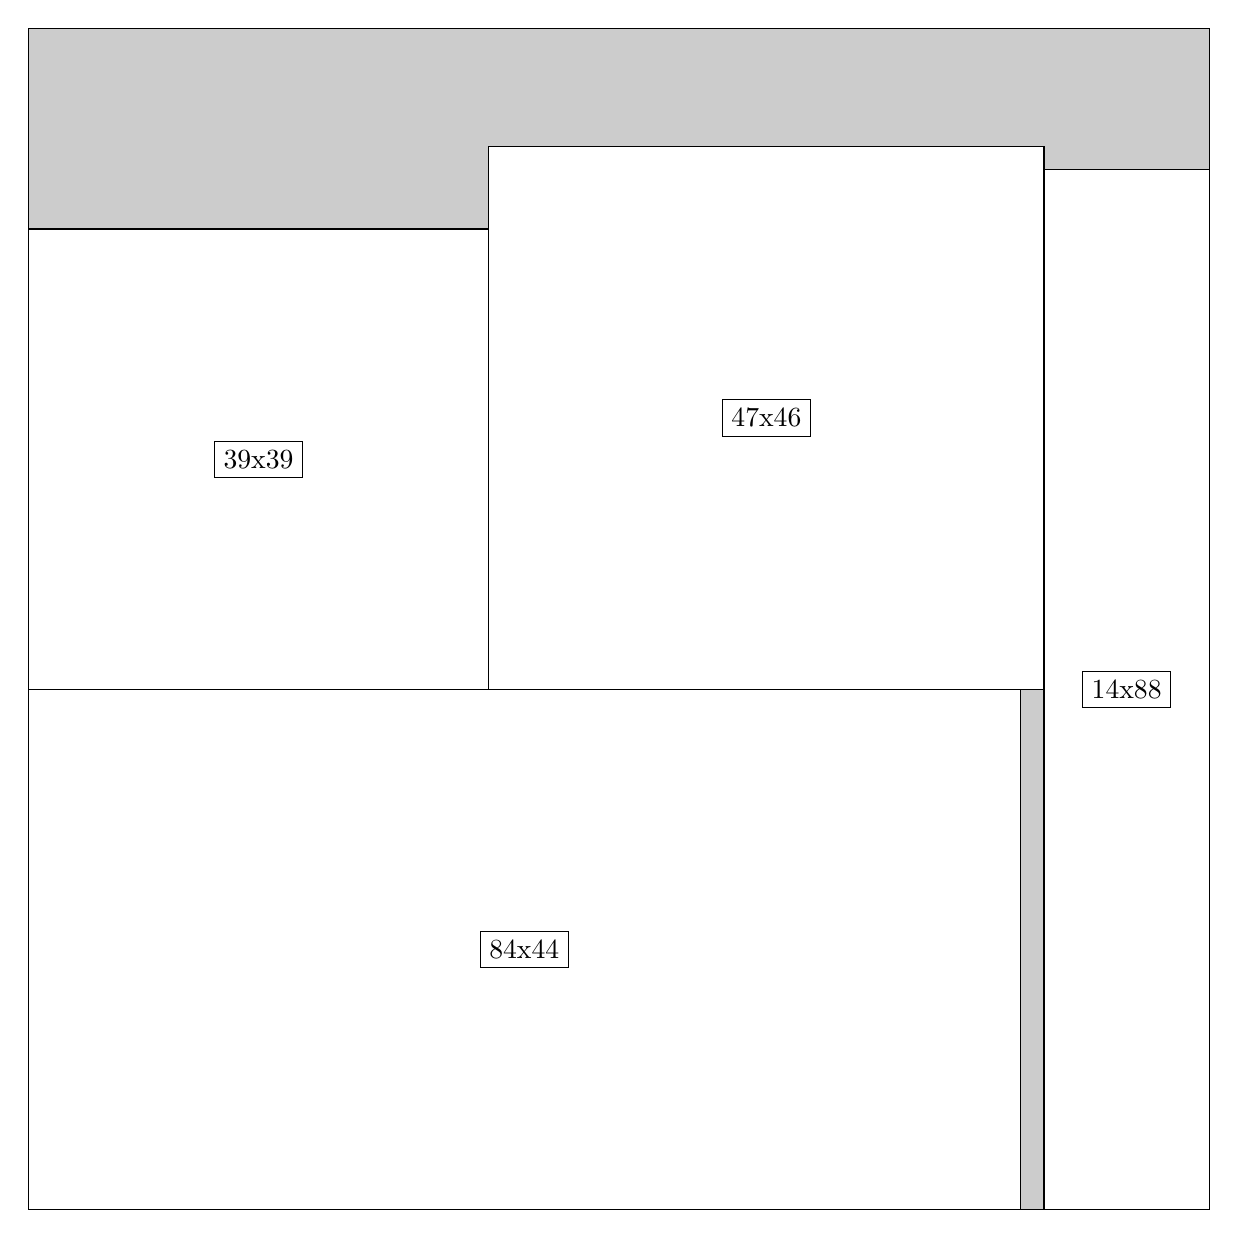
\begin{tikzpicture}[shorten >=1pt,scale=1.0,every node/.style={scale=1.0},->]
\tikzstyle{vertex}=[circle,fill=black!25,minimum size=14pt,inner sep=0pt]
\filldraw[fill=gray!40!white, draw=black] (0,0) rectangle (15.0,15.0);
\foreach \name/\x/\y/\w/\h in {84x44/0.0/0.0/12.6/6.6,47x46/5.85/6.6/7.05/6.8999999999999995,39x39/0.0/6.6/5.85/5.85,14x88/12.9/0.0/2.1/13.2}
\filldraw[fill=white!40!white, draw=black] (\x,\y) rectangle node[draw] (\name) {\name} ++(\w,\h);
\end{tikzpicture}


w =84 , h =44 , x =0 , y =0 , v =3696
\par
w =47 , h =46 , x =39 , y =44 , v =2162
\par
w =39 , h =39 , x =0 , y =44 , v =1521
\par
w =14 , h =88 , x =86 , y =0 , v =1232
\par
\newpage


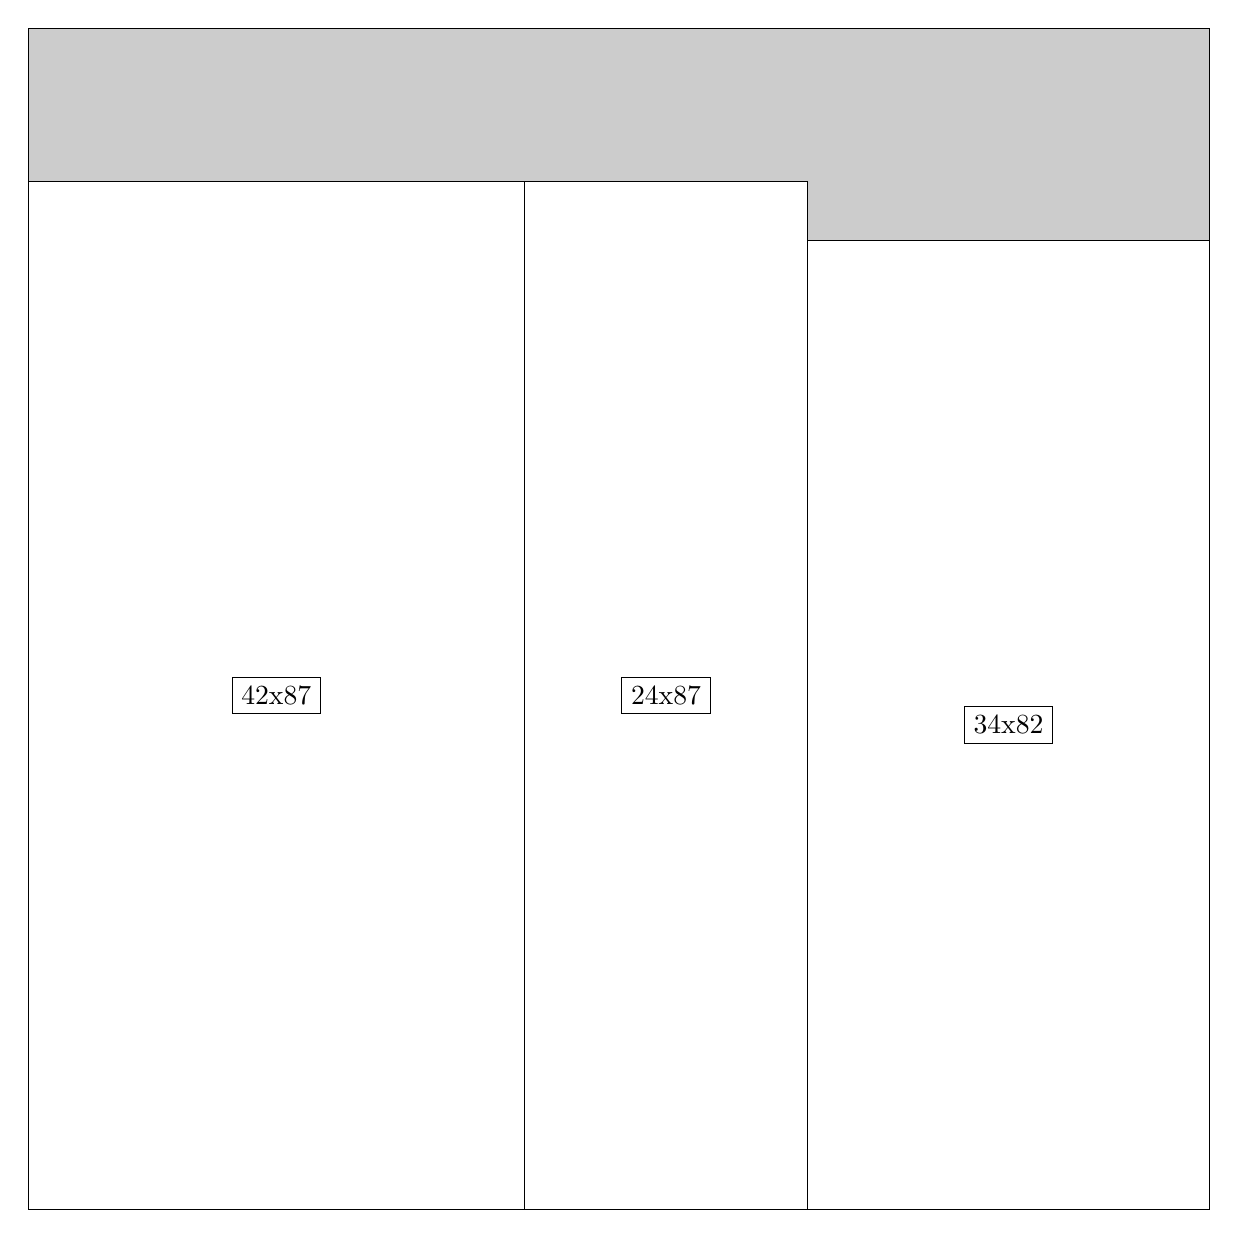
\begin{tikzpicture}[shorten >=1pt,scale=1.0,every node/.style={scale=1.0},->]
\tikzstyle{vertex}=[circle,fill=black!25,minimum size=14pt,inner sep=0pt]
\filldraw[fill=gray!40!white, draw=black] (0,0) rectangle (15.0,15.0);
\foreach \name/\x/\y/\w/\h in {42x87/0.0/0.0/6.3/13.049999999999999,34x82/9.9/0.0/5.1/12.299999999999999,24x87/6.3/0.0/3.5999999999999996/13.049999999999999}
\filldraw[fill=white!40!white, draw=black] (\x,\y) rectangle node[draw] (\name) {\name} ++(\w,\h);
\end{tikzpicture}


w =42 , h =87 , x =0 , y =0 , v =3654
\par
w =34 , h =82 , x =66 , y =0 , v =2788
\par
w =24 , h =87 , x =42 , y =0 , v =2088
\par
\newpage


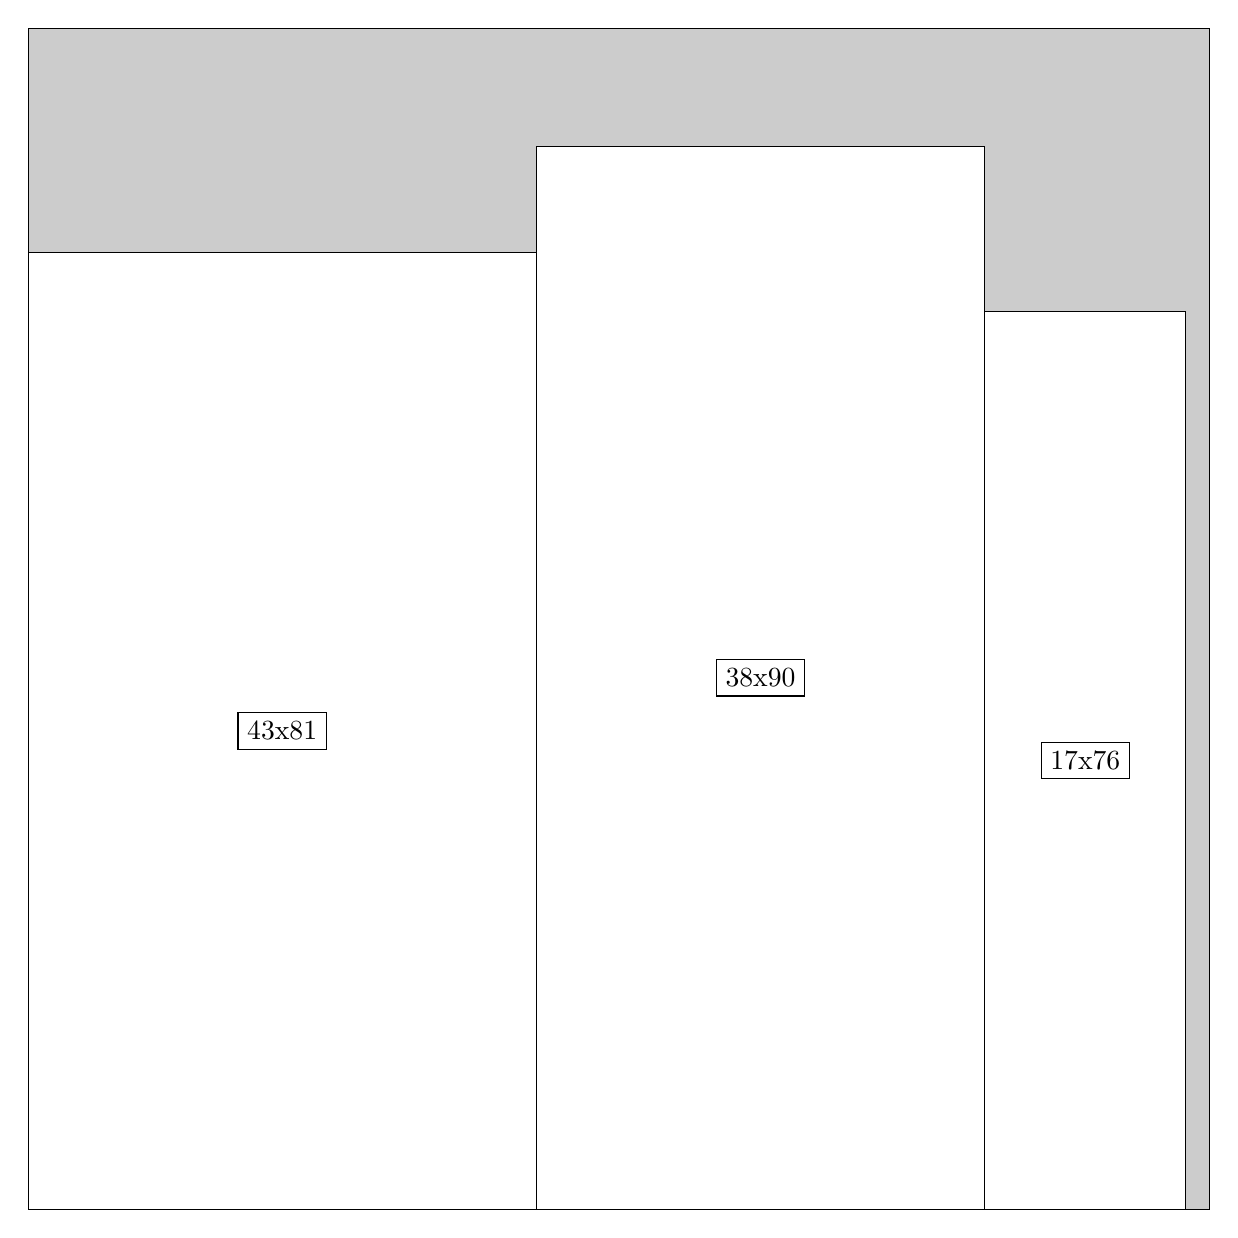
\begin{tikzpicture}[shorten >=1pt,scale=1.0,every node/.style={scale=1.0},->]
\tikzstyle{vertex}=[circle,fill=black!25,minimum size=14pt,inner sep=0pt]
\filldraw[fill=gray!40!white, draw=black] (0,0) rectangle (15.0,15.0);
\foreach \name/\x/\y/\w/\h in {43x81/0.0/0.0/6.45/12.15,38x90/6.45/0.0/5.7/13.5,17x76/12.15/0.0/2.55/11.4}
\filldraw[fill=white!40!white, draw=black] (\x,\y) rectangle node[draw] (\name) {\name} ++(\w,\h);
\end{tikzpicture}


w =43 , h =81 , x =0 , y =0 , v =3483
\par
w =38 , h =90 , x =43 , y =0 , v =3420
\par
w =17 , h =76 , x =81 , y =0 , v =1292
\par
\newpage


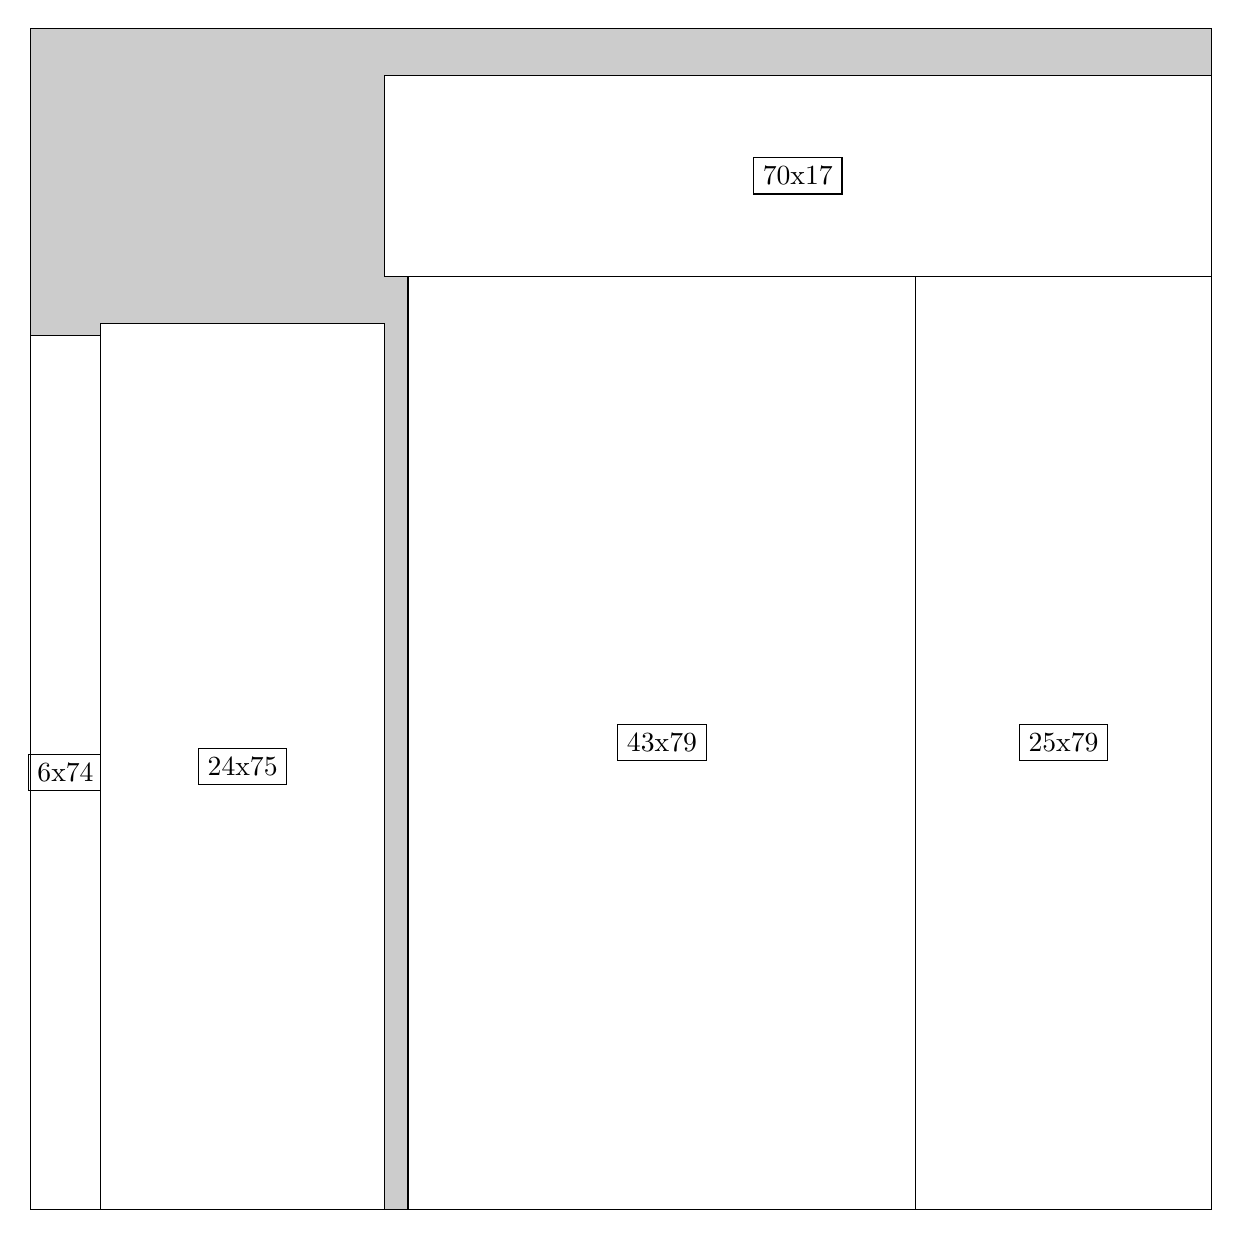
\begin{tikzpicture}[shorten >=1pt,scale=1.0,every node/.style={scale=1.0},->]
\tikzstyle{vertex}=[circle,fill=black!25,minimum size=14pt,inner sep=0pt]
\filldraw[fill=gray!40!white, draw=black] (0,0) rectangle (15.0,15.0);
\foreach \name/\x/\y/\w/\h in {6x74/0.0/0.0/0.8999999999999999/11.1,25x79/11.25/0.0/3.75/11.85,24x75/0.8999999999999999/0.0/3.5999999999999996/11.25,70x17/4.5/11.85/10.5/2.55,43x79/4.8/0.0/6.45/11.85}
\filldraw[fill=white!40!white, draw=black] (\x,\y) rectangle node[draw] (\name) {\name} ++(\w,\h);
\end{tikzpicture}


w =6 , h =74 , x =0 , y =0 , v =444
\par
w =25 , h =79 , x =75 , y =0 , v =1975
\par
w =24 , h =75 , x =6 , y =0 , v =1800
\par
w =70 , h =17 , x =30 , y =79 , v =1190
\par
w =43 , h =79 , x =32 , y =0 , v =3397
\par
\newpage


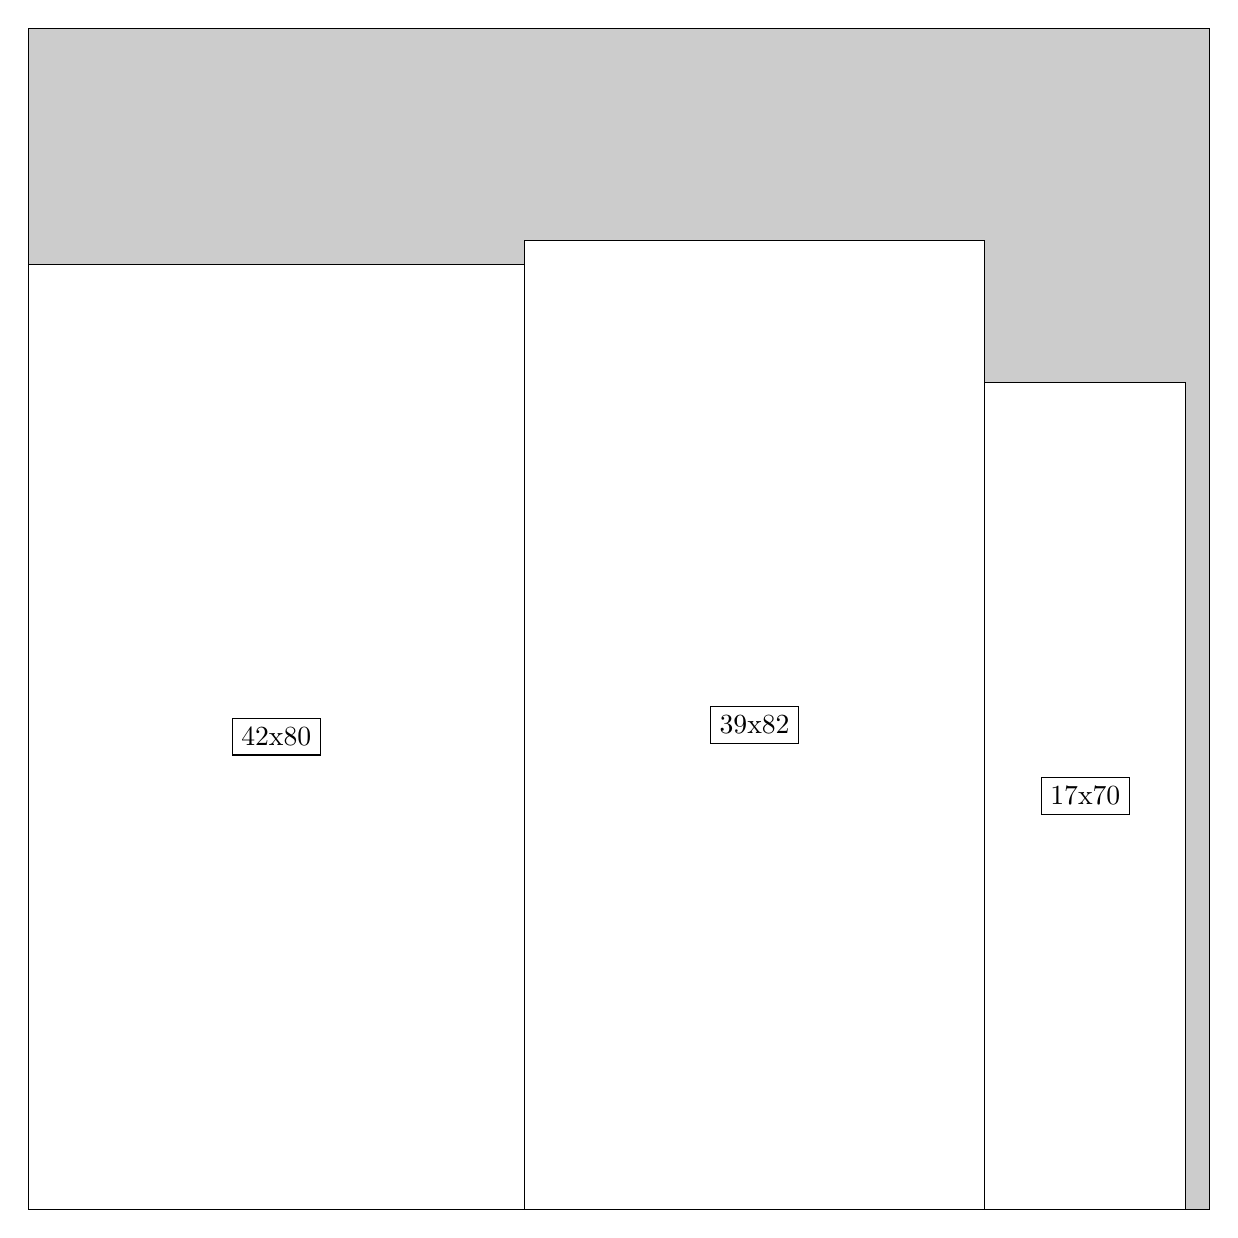
\begin{tikzpicture}[shorten >=1pt,scale=1.0,every node/.style={scale=1.0},->]
\tikzstyle{vertex}=[circle,fill=black!25,minimum size=14pt,inner sep=0pt]
\filldraw[fill=gray!40!white, draw=black] (0,0) rectangle (15.0,15.0);
\foreach \name/\x/\y/\w/\h in {42x80/0.0/0.0/6.3/12.0,39x82/6.3/0.0/5.85/12.299999999999999,17x70/12.15/0.0/2.55/10.5}
\filldraw[fill=white!40!white, draw=black] (\x,\y) rectangle node[draw] (\name) {\name} ++(\w,\h);
\end{tikzpicture}


w =42 , h =80 , x =0 , y =0 , v =3360
\par
w =39 , h =82 , x =42 , y =0 , v =3198
\par
w =17 , h =70 , x =81 , y =0 , v =1190
\par
\newpage


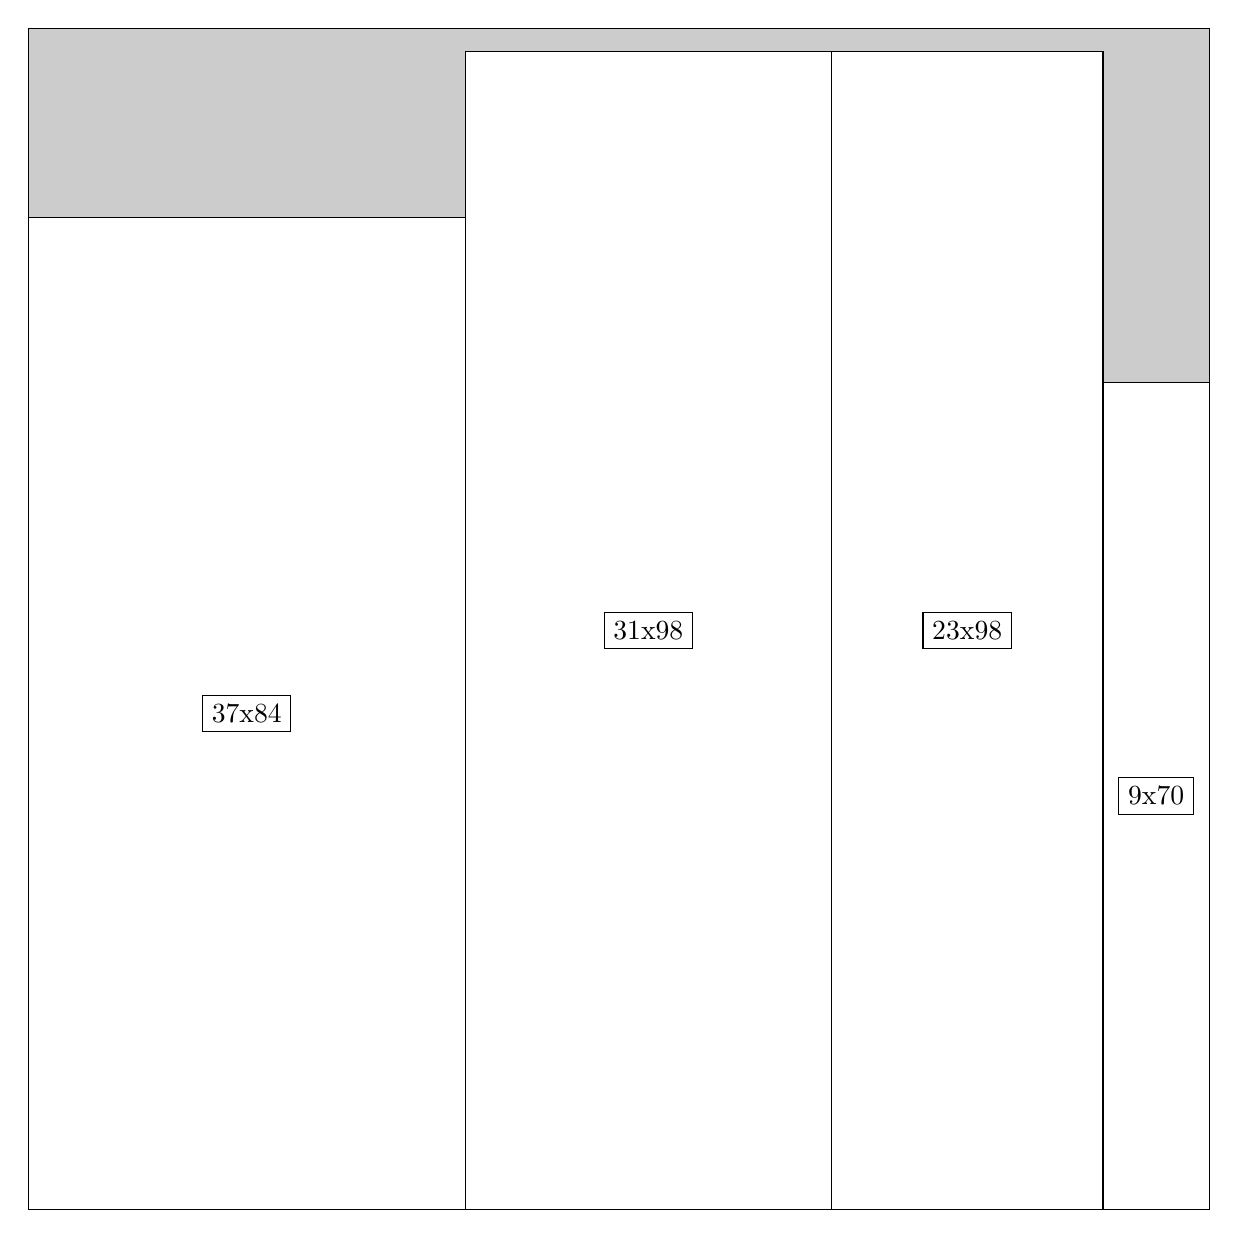
\begin{tikzpicture}[shorten >=1pt,scale=1.0,every node/.style={scale=1.0},->]
\tikzstyle{vertex}=[circle,fill=black!25,minimum size=14pt,inner sep=0pt]
\filldraw[fill=gray!40!white, draw=black] (0,0) rectangle (15.0,15.0);
\foreach \name/\x/\y/\w/\h in {37x84/0.0/0.0/5.55/12.6,31x98/5.55/0.0/4.6499999999999995/14.7,23x98/10.2/0.0/3.4499999999999997/14.7,9x70/13.65/0.0/1.3499999999999999/10.5}
\filldraw[fill=white!40!white, draw=black] (\x,\y) rectangle node[draw] (\name) {\name} ++(\w,\h);
\end{tikzpicture}


w =37 , h =84 , x =0 , y =0 , v =3108
\par
w =31 , h =98 , x =37 , y =0 , v =3038
\par
w =23 , h =98 , x =68 , y =0 , v =2254
\par
w =9 , h =70 , x =91 , y =0 , v =630
\par
\newpage


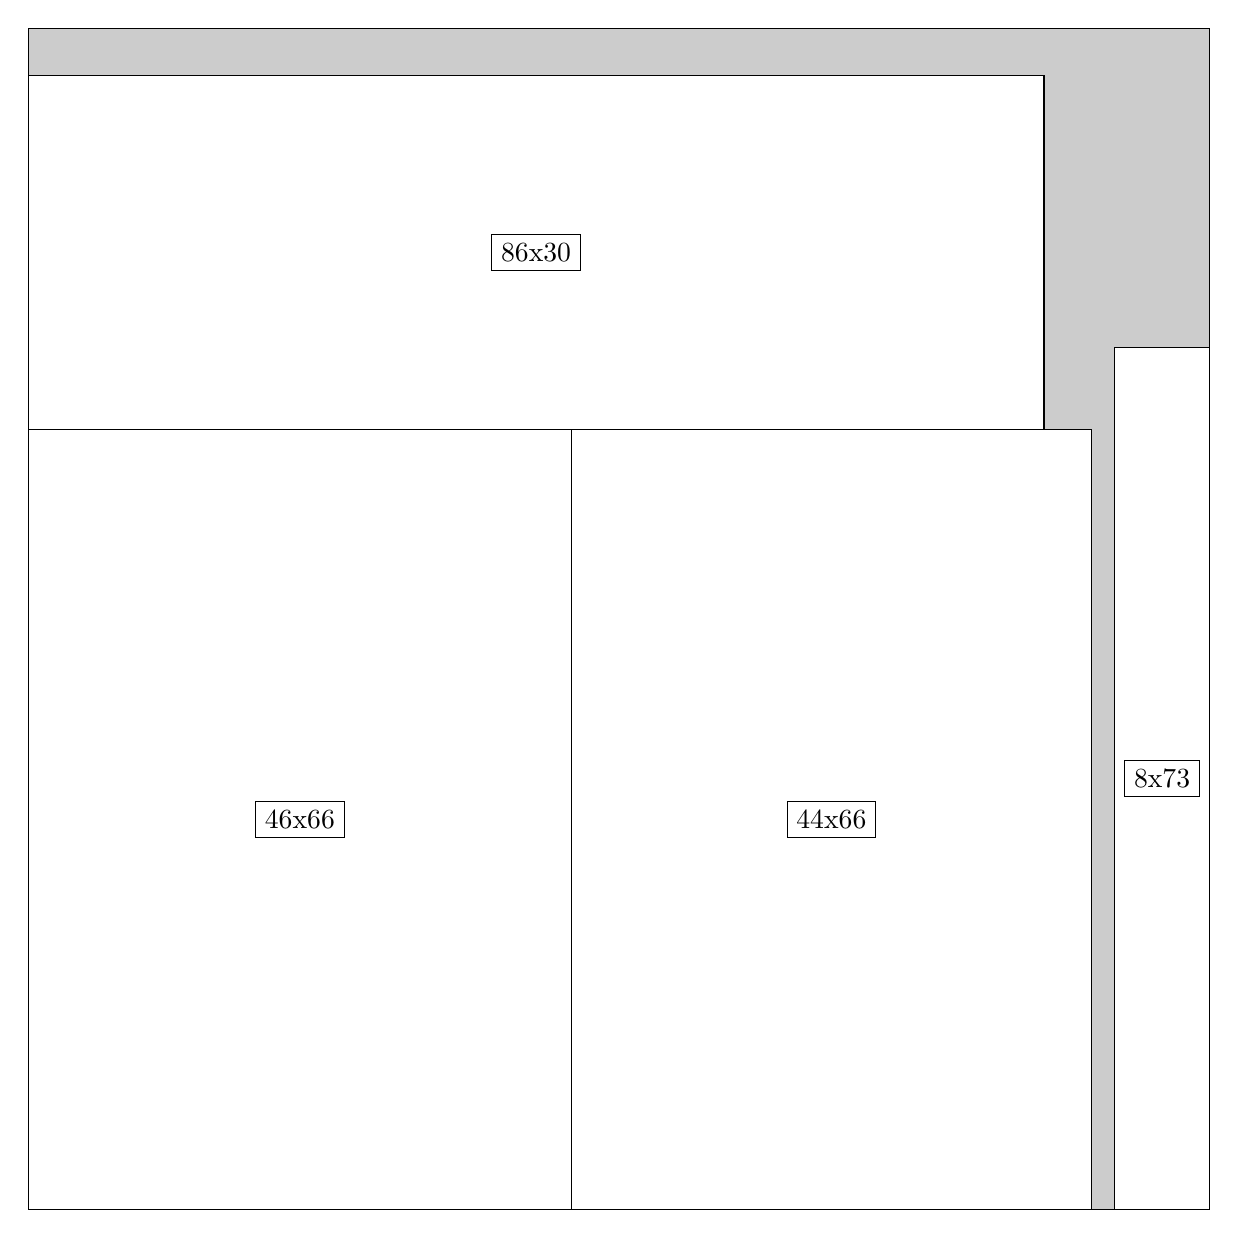
\begin{tikzpicture}[shorten >=1pt,scale=1.0,every node/.style={scale=1.0},->]
\tikzstyle{vertex}=[circle,fill=black!25,minimum size=14pt,inner sep=0pt]
\filldraw[fill=gray!40!white, draw=black] (0,0) rectangle (15.0,15.0);
\foreach \name/\x/\y/\w/\h in {46x66/0.0/0.0/6.8999999999999995/9.9,44x66/6.8999999999999995/0.0/6.6/9.9,86x30/0.0/9.9/12.9/4.5,8x73/13.799999999999999/0.0/1.2/10.95}
\filldraw[fill=white!40!white, draw=black] (\x,\y) rectangle node[draw] (\name) {\name} ++(\w,\h);
\end{tikzpicture}


w =46 , h =66 , x =0 , y =0 , v =3036
\par
w =44 , h =66 , x =46 , y =0 , v =2904
\par
w =86 , h =30 , x =0 , y =66 , v =2580
\par
w =8 , h =73 , x =92 , y =0 , v =584
\par
\newpage


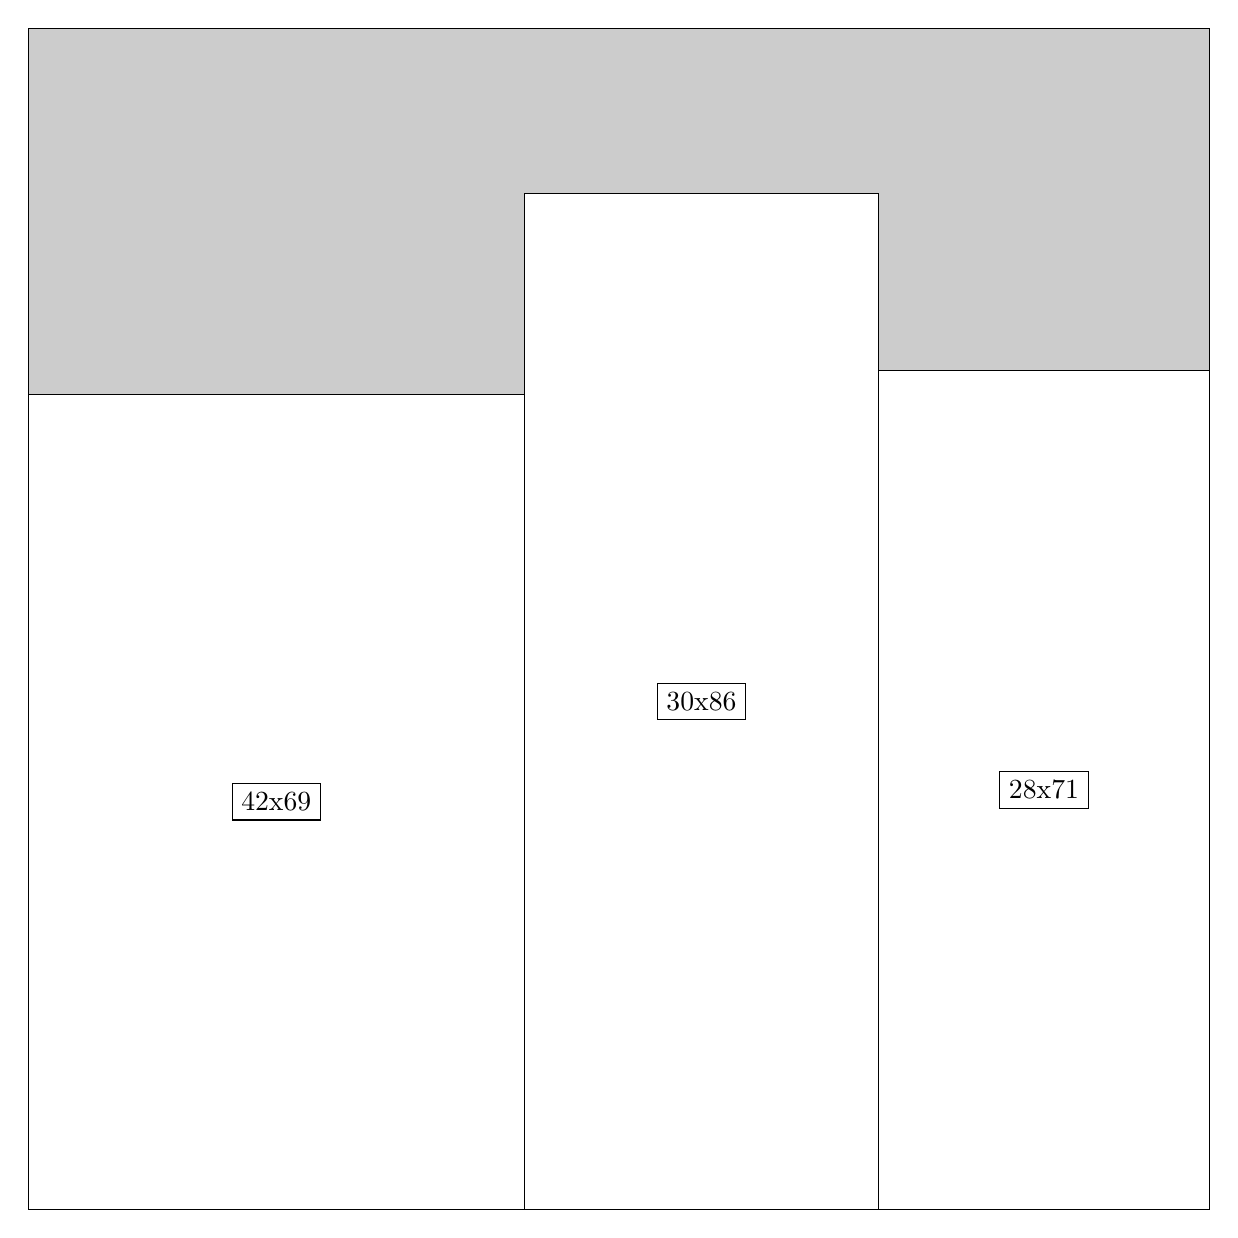
\begin{tikzpicture}[shorten >=1pt,scale=1.0,every node/.style={scale=1.0},->]
\tikzstyle{vertex}=[circle,fill=black!25,minimum size=14pt,inner sep=0pt]
\filldraw[fill=gray!40!white, draw=black] (0,0) rectangle (15.0,15.0);
\foreach \name/\x/\y/\w/\h in {42x69/0.0/0.0/6.3/10.35,30x86/6.3/0.0/4.5/12.9,28x71/10.799999999999999/0.0/4.2/10.65}
\filldraw[fill=white!40!white, draw=black] (\x,\y) rectangle node[draw] (\name) {\name} ++(\w,\h);
\end{tikzpicture}


w =42 , h =69 , x =0 , y =0 , v =2898
\par
w =30 , h =86 , x =42 , y =0 , v =2580
\par
w =28 , h =71 , x =72 , y =0 , v =1988
\par
\newpage


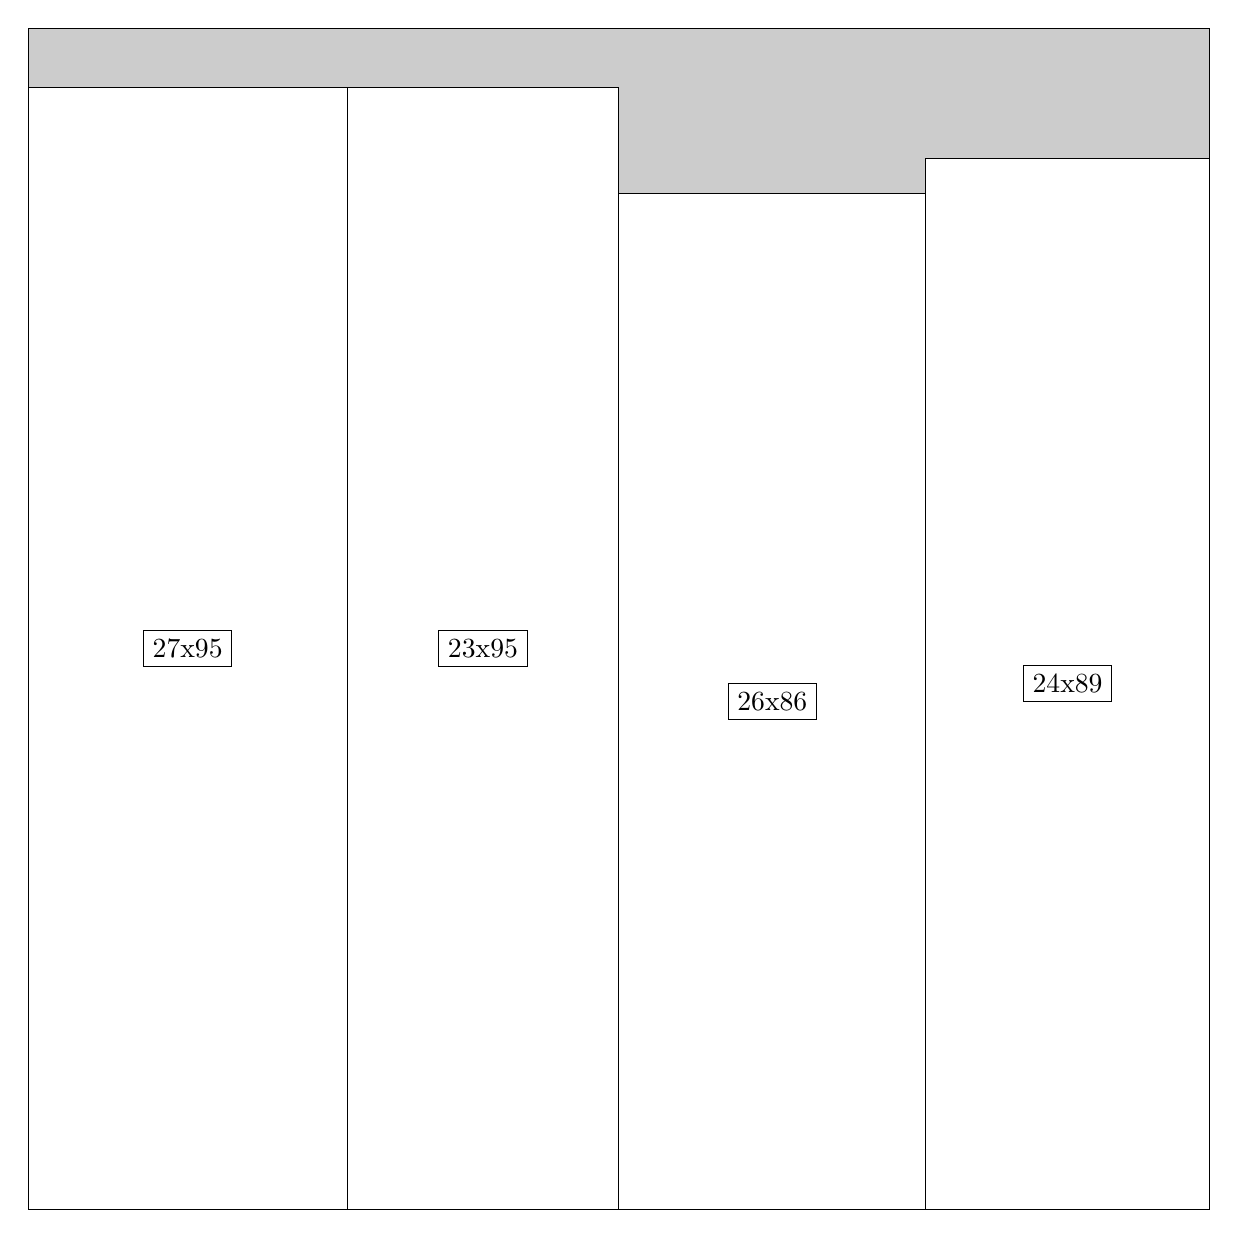
\begin{tikzpicture}[shorten >=1pt,scale=1.0,every node/.style={scale=1.0},->]
\tikzstyle{vertex}=[circle,fill=black!25,minimum size=14pt,inner sep=0pt]
\filldraw[fill=gray!40!white, draw=black] (0,0) rectangle (15.0,15.0);
\foreach \name/\x/\y/\w/\h in {27x95/0.0/0.0/4.05/14.25,26x86/7.5/0.0/3.9/12.9,23x95/4.05/0.0/3.4499999999999997/14.25,24x89/11.4/0.0/3.5999999999999996/13.35}
\filldraw[fill=white!40!white, draw=black] (\x,\y) rectangle node[draw] (\name) {\name} ++(\w,\h);
\end{tikzpicture}


w =27 , h =95 , x =0 , y =0 , v =2565
\par
w =26 , h =86 , x =50 , y =0 , v =2236
\par
w =23 , h =95 , x =27 , y =0 , v =2185
\par
w =24 , h =89 , x =76 , y =0 , v =2136
\par
\newpage


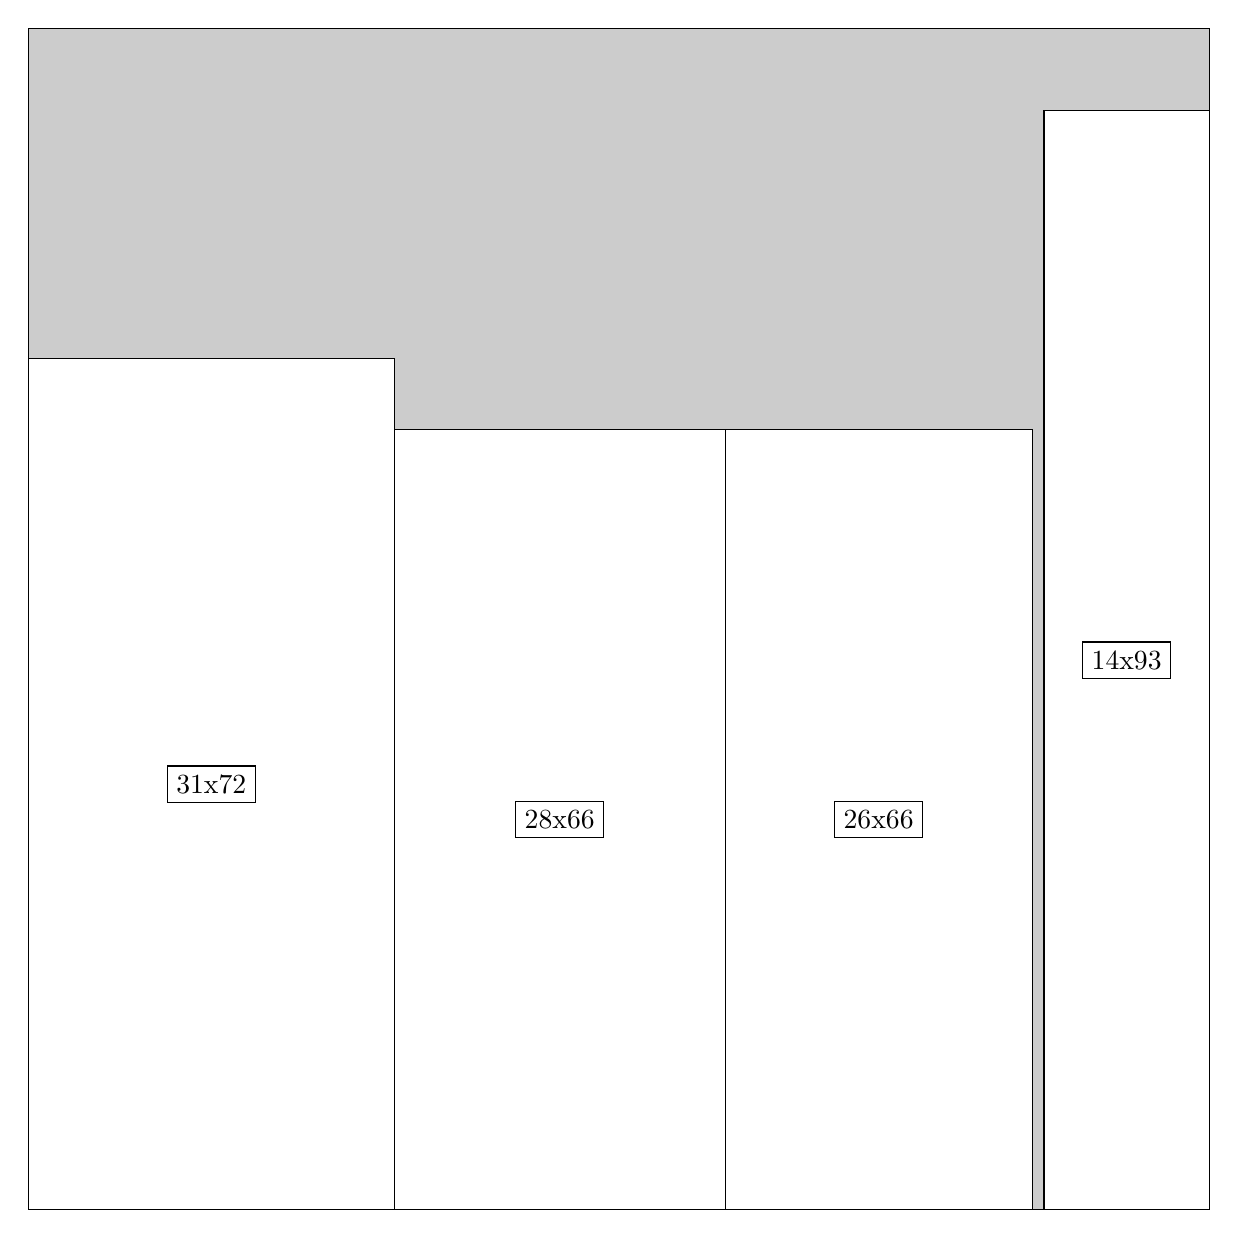
\begin{tikzpicture}[shorten >=1pt,scale=1.0,every node/.style={scale=1.0},->]
\tikzstyle{vertex}=[circle,fill=black!25,minimum size=14pt,inner sep=0pt]
\filldraw[fill=gray!40!white, draw=black] (0,0) rectangle (15.0,15.0);
\foreach \name/\x/\y/\w/\h in {31x72/0.0/0.0/4.6499999999999995/10.799999999999999,28x66/4.6499999999999995/0.0/4.2/9.9,26x66/8.85/0.0/3.9/9.9,14x93/12.9/0.0/2.1/13.95}
\filldraw[fill=white!40!white, draw=black] (\x,\y) rectangle node[draw] (\name) {\name} ++(\w,\h);
\end{tikzpicture}


w =31 , h =72 , x =0 , y =0 , v =2232
\par
w =28 , h =66 , x =31 , y =0 , v =1848
\par
w =26 , h =66 , x =59 , y =0 , v =1716
\par
w =14 , h =93 , x =86 , y =0 , v =1302
\par
\newpage


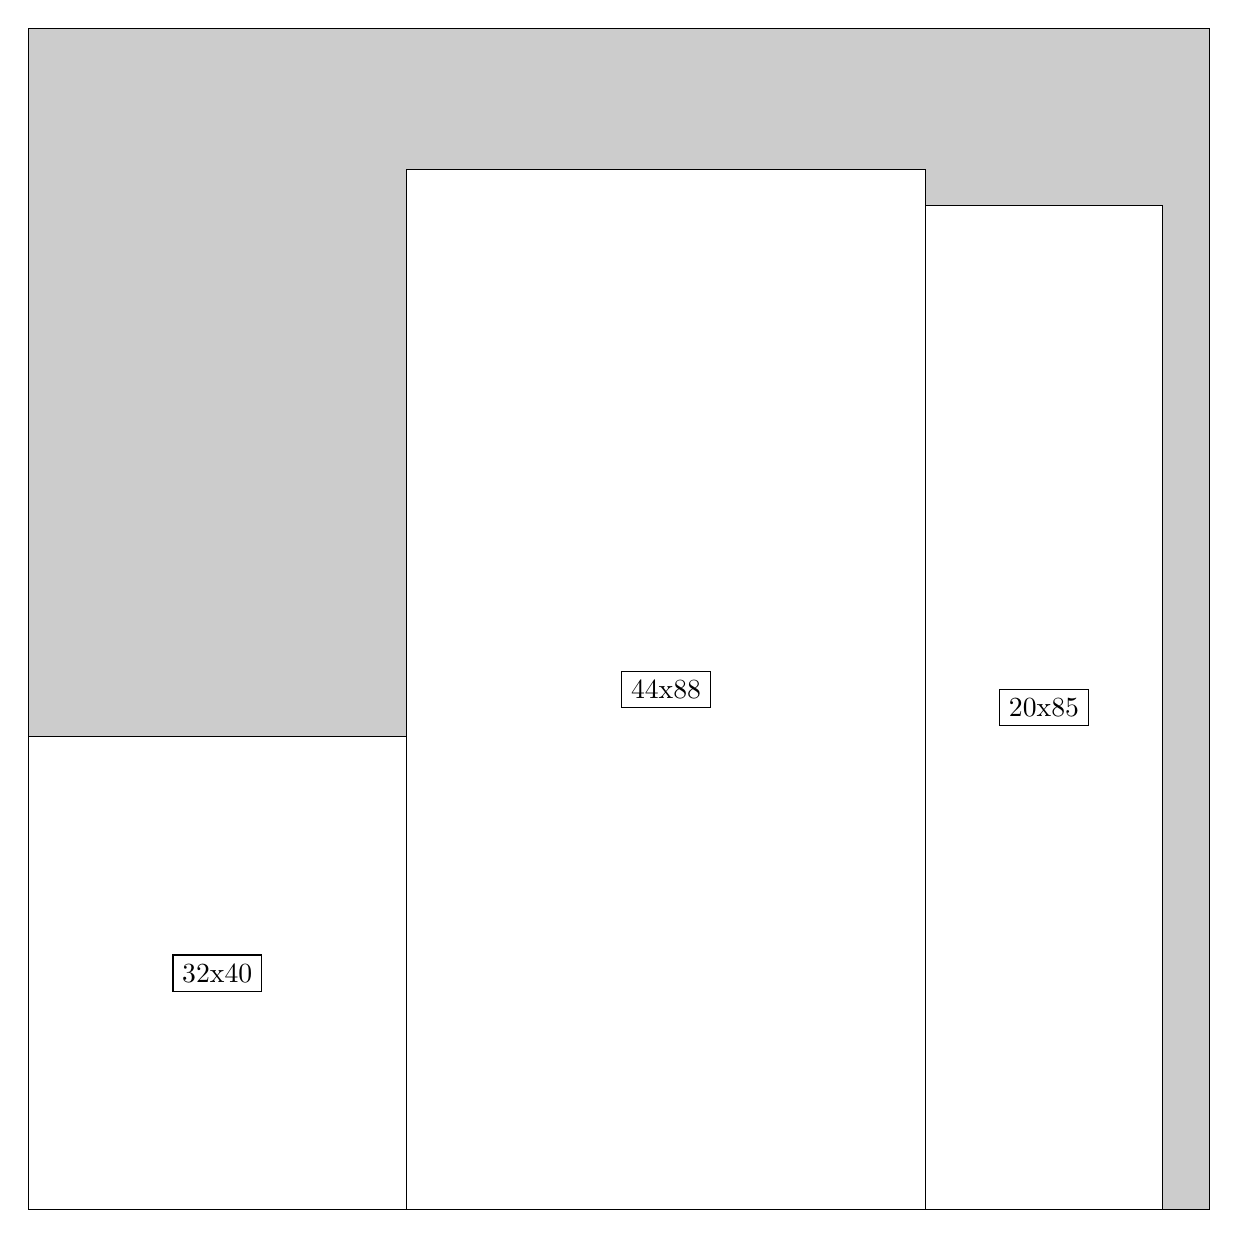
\begin{tikzpicture}[shorten >=1pt,scale=1.0,every node/.style={scale=1.0},->]
\tikzstyle{vertex}=[circle,fill=black!25,minimum size=14pt,inner sep=0pt]
\filldraw[fill=gray!40!white, draw=black] (0,0) rectangle (15.0,15.0);
\foreach \name/\x/\y/\w/\h in {44x88/4.8/0.0/6.6/13.2,20x85/11.4/0.0/3.0/12.75,32x40/0.0/0.0/4.8/6.0}
\filldraw[fill=white!40!white, draw=black] (\x,\y) rectangle node[draw] (\name) {\name} ++(\w,\h);
\end{tikzpicture}


w =44 , h =88 , x =32 , y =0 , v =3872
\par
w =20 , h =85 , x =76 , y =0 , v =1700
\par
w =32 , h =40 , x =0 , y =0 , v =1280
\par
\newpage


\end{document}